% Main paper; full.tex adds the unchanged appendix for the reading version.
\documentclass{article}
\usepackage{iclr2027_conference,times}
\usepackage[T1]{fontenc}
\usepackage[utf8]{inputenc}
\usepackage{microtype}
\usepackage{amsmath,amssymb,amsthm,bm}
\usepackage{booktabs,multirow,tabularx,array}
\usepackage{graphicx,float,placeins,lscape}
\usepackage{xcolor,listings}
\usepackage{url}
\usepackage{xr-hyper}
\usepackage[hidelinks]{hyperref}
\usepackage[nameinlink,noabbrev]{cleveref}
\usepackage{enumitem}
\usepackage{seqsplit}

\newtheorem{proposition}{Proposition}
\graphicspath{{figures/}}
\newcommand{\code}[1]{\texttt{#1}}
\newcommand{\codebrk}[1]{\texttt{\small\seqsplit{#1}}}
\newcommand{\stdmax}{\ensuremath{\sigma_{\max}}}
\newcommand{\vTwoNumberMacros}{tables/multiseverity_numbers}
\newcommand{\vTwoAssociationTable}{tables/table_multiseverity_associations}
\newcommand{\vTwoDecisionTable}{tables/table_multiseverity_decisions}
\newcommand{\vTwoSRLabelReference}{\Cref{tab:sr-labels}}
\newcommand{\blindsubmission}{}
\input{\vTwoNumberMacros}

\title{Diagnosing JEPA World Models with Action-Conditioned Predictive Consistency}
\author{Anonymous Authors}
\hypersetup{
  pdftitle={Diagnosing JEPA World Models with Action-Conditioned Predictive Consistency},
  pdfauthor={}
}


% Import section/figure labels without importing another PDF's bibliography.
\newcommand{\acpcExternalDocument}[1]{%
  \IfFileExists{build/#1.aux}{%
    \externaldocument[][nocite]{build/#1}[#1.pdf]%
  }{%
    \externaldocument[][nocite]{#1}[#1.pdf]%
  }%
}
% Keep appendix figure, table, equation and proposition numbers consistent.
\makeatletter
\newcommand{\acpcSaveMainCounters}{%
  \begingroup
  \edef\@currentlabel{\arabic{figure}}\label{acpc:main-figures}%
  \edef\@currentlabel{\arabic{table}}\label{acpc:main-tables}%
  \edef\@currentlabel{\arabic{equation}}\label{acpc:main-equations}%
  \edef\@currentlabel{\arabic{proposition}}\label{acpc:main-propositions}%
  \endgroup
}
\makeatother
\newcommand{\acpcRestoreMainCounters}{%
  \setcounter{figure}{\getrefnumber{acpc:main-figures}}%
  \setcounter{table}{\getrefnumber{acpc:main-tables}}%
  \setcounter{equation}{\getrefnumber{acpc:main-equations}}%
  \setcounter{proposition}{\getrefnumber{acpc:main-propositions}}%
}

\ifdefined\ACPCFull
\else
  \acpcExternalDocument{supplementary}
\fi
\begin{document}
\maketitle

\begin{abstract}
Joint-embedding predictive architectures (JEPAs) learn world models that
predict in a compact latent space rather than in pixels, reducing the
pressure to model nuisance appearance. Yet this provides no guarantee against visual perturbations: they can
still alter the encoded representation and affect subsequent
action-conditioned predictions.
Bisimulation captures this requirement precisely: two observations should be
treated as the same state only when their action-conditioned consequences
agree. Guided by this criterion, we introduce Action-Conditioned Predictive
Consistency (ACPC), a diagnostic that measures how far a clean history and
a visually perturbed view of it diverge after being rolled forward under the
same action sequence. We prove that this divergence bounds perturbation-induced changes in multi-step prediction error and planner cost, i.e., the change in predicted cost caused by a visual perturbation under the same action sequence. Building on pairwise ACPC, we define two complementary measures: Invariance Radius (IR) summarizes clean--perturbed rollout spread, while Separation Rate (SR) checks whether different states remain distinguishable after rollout.
Experiments on four visual control tasks show that pairwise ACPC predicts perturbation-induced changes in prediction error and planner cost. On LeWM, the joint IR--SR screen
transfers across tasks, and both IR and SR remain informative under blur and
resize. PLDM exhibits similar diagnostic trends
under a different architecture.\ifdefined\blindsubmission\else\
Code is available \href{\paperpubliccodeurl}{\textcolor{blue}{here}}.\fi

\end{abstract}

%% ===========================================================================
\section{Introduction}\label{sec:intro}

World models support control by predicting the outcomes of candidate
actions~\citep{hafner2025dreamerv3,hansen2024tdmpc2}. Joint-embedding
predictive architectures (JEPAs) predict target representations in a latent space rather than
reconstructing pixels, avoiding an explicit requirement to reproduce nuisance
visual details
~\citep{lecun2022path,assran2023ijepa,bardes2024vjepa,vanassel2025jointembeddingreconstruction,littwin2024jepaavoidsnoisyfeatures}.
Yet this design alone does not determine which visual differences matter for
control.
Such representations should be insensitive to task-irrelevant visual
perturbations while preserving distinctions between situations that require
different actions.
This requirement echoes the intuition behind bisimulation, which defines
state equivalence through action-conditioned consequences rather than visual
appearance~\citep{gelada2019deepmdp,zhang2021dbc}. However, initial representation distances
alone do not show how a perturbation propagates through prediction. Over a
multi-step rollout, the predictor may amplify or contract the initial
representation difference. Encoder-level and single-step diagnostics
do not directly measure this rollout-level effect. We therefore ask: when a
clean history and its perturbed view are rolled forward under the same action
sequence, how far apart are their predicted trajectories?

To measure this rollout-level effect, we introduce Action-Conditioned
Predictive Consistency (ACPC). ACPC rolls a clean history and its perturbed
view forward under the same action sequence and measures the distance between
their predicted trajectories. \Cref{fig:acpc-ir-sr-overview} provides a
conceptual overview of how this pairwise distance is summarized by \emph{Invariance Radius} (IR) and
complemented by \emph{Separation Rate} (SR). Low ACPC alone, however, does not rule out representational collapse: a constant representation would make every paired
rollout identical. We therefore summarize ACPC values across histories with IR, where lower values indicate less sensitivity
to visual perturbations. SR checks whether different states remain distinguishable after being rolled forward, with higher values
indicating better separation.

\begin{figure}[t]
\centering
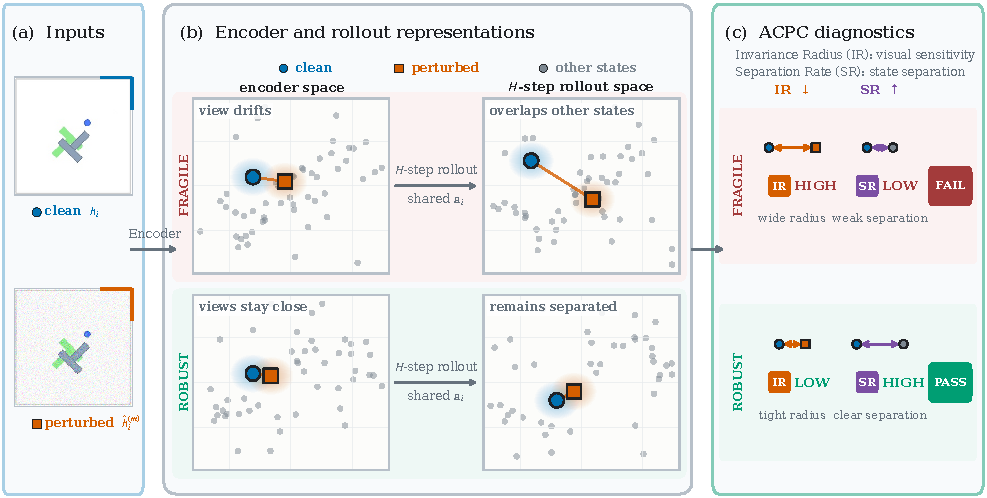
\includegraphics[width=1.00\linewidth]{fig_acpc_ir_sr_overview.pdf}
\caption{\textbf{Conceptual overview of ACPC, IR, and SR.}
\textbf{(a)}~A logged clean history and a visually perturbed view of it form
the paired inputs. \textbf{(b)}~A frozen world model encodes both views and
rolls them forward for $H$ steps under the same recorded action sequence. ACPC
measures the distance between the two predicted trajectories.
\textbf{(c)}~IR summarizes perturbation-induced rollout
spread across histories, while SR measures how often
selected different-state rollouts remain separated beyond this spread.
}
\label{fig:acpc-ir-sr-overview}
\end{figure}

We make three contributions. First, we introduce \textbf{ACPC}, which compares
clean and perturbed rollout predictions under shared actions; IR summarizes
sensitivity and SR checks state separation (\Cref{sec:acpc}). Second, we
prove samplewise \textbf{bounds on prediction-error and planning-cost changes}
over multi-step rollouts in which the same candidate action sequences are applied to both views
(\Cref{prop:target-free-error-drift,prop:exact-cost-certificate}). These bounds
require no distributional or smoothness assumptions. Third, we develop
\textbf{ACPC-based checkpoint screening} using both IR and SR and evaluate the three proposed diagnostics on four tasks, three visual perturbations, and two architectures.
On LeWM~\citep{maes2026lewm}, ACPC is informative about perturbation-induced changes in prediction error and in the action sequences selected by the cross-entropy method (CEM~\citep{kroese2006cem}). Across
checkpoints, IR and SR provide non-equivalent views of perturbation sensitivity
and state separation; their continuous values covary with retained
control performance (\Cref{sec:exp}).

\section{Related Work}\label{sec:related}

\paragraph{World Models.}
World models predict how an environment evolves under actions and use those
predictions for control. DreamerV3~\citep{hafner2025dreamerv3} learns from
imagined trajectories, while TD-MPC2~\citep{hansen2024tdmpc2} plans with
learned latent dynamics. JEPAs
learn representations by predicting targets in a latent space rather
than reconstructing pixels
~\citep{lecun2022path,assran2023ijepa,bardes2024vjepa,assran2025vjepa2}.
For goal-conditioned planning, PLDM~\citep{sobal2025stresstesting} learns
action-conditioned latent dynamics from reward-free offline data using
VICReg-inspired regularization.
LeWM~\citep{maes2026lewm} is an end-to-end JEPA world model for
action-conditioned latent prediction with a simple two-term objective: a
next-step latent prediction loss and LeJEPA's SIGReg~\citep{balestriero2025lejepa}, which serves as the sole anti-collapse regularizer.
Related work studies collapse in self-predictive
learning~\citep{tang2023selfpredictive}.
VICReg~\citep{bardes2022vicreg} prevents representation collapse with variance regularization
and reduces feature redundancy with covariance regularization.
VISReg~\citep{wu2026visreg} retains variance regularization but
replaces VICReg's covariance regularization with Sliced-Wasserstein-based
sketching.
Complementary work studies the role of action
conditioning~\citep{khetarpal2025actionconditional}.
Theoretical analyses ask which features latent prediction retains
~\citep{vanassel2025jointembeddingreconstruction,littwin2024jepaavoidsnoisyfeatures}.
seq-JEPA~\citep{ghaemi2025seqjepa} further studies invariance and equivariance
under known view transformations.

\paragraph{Robustness to Visual Perturbations.}
A common approach is to make learned representations insensitive to nuisance
appearance changes during training. DrQ~\citep{kostrikov2020drq} and
DrQ-v2~\citep{yarats2022drqv2} use image augmentation to reduce visual
overfitting in pixel-based control, while SODA~\citep{hansen2021soda}
decouples augmentation from policy learning and uses it to train invariant
visual representations. ReOI~\citep{chen2025reoi} instead intervenes at test
time, removing detected visual distractors before world-model prediction and
then reintroducing them after prediction.
Other methods modify what the world model is encouraged to represent.
DreamerPro~\citep{deng2022dreamerpro} replaces pixel reconstruction with
prototypical representation learning to reduce sensitivity to background
distractors. Denoised MDPs~\citep{wang2022denoisedmdps} explicitly separate
control- and reward-relevant information from nuisance factors, while
\citet{sun2024latentrobustwm} combine spatio-temporal masking with
bisimulation-based representation learning to suppress exogenous visual noise.
These approaches reflect a common principle: reducing the influence of visual
differences that do not affect control while preserving distinctions that do.
Bisimulation formalizes this principle by treating states as behaviorally
similar when the same actions lead to similar rewards and transition
dynamics~\citep{gelada2019deepmdp,zhang2021dbc,bsmpc}. Recent JEPA-based work
adapts this idea to reward-free planning by defining state similarity from
transition dynamics alone~\citep{toso2026bisimjepa}.
In a related training-time approach, MWM~\citep{yan2026mwm} uses post-training to improve action-conditioned
consistency over multi-step world-model predictions.


\paragraph{Diagnostics for World Models.}
Model accuracy does not necessarily predict control performance:
one-step likelihood can be poorly correlated with downstream
performance~\citep{lambert2020objective}.
This objective mismatch has motivated decision-aware approaches to model
learning and evaluation~\citep{wei2024objectivemismatch}.
More broadly, world-model evaluation should match the model's intended
decision-making use rather than rely on prediction fidelity
alone~\citep{yu2026worldmodelevaluation}.
Recent diagnostics examine different aspects of decision-relevant world-model
behavior. ATM~\citep{chen2026atm} compares action information in encoded
environment transitions and model-predicted transitions. Inverse-dynamics
probes measure how well actions can be recovered from learned
latents~\citep{yeom2026actionrelevant}. At the rollout level,
\citet{schaefer2026kinematic} test whether long imagined rollouts respond to
changes in physical dynamics rather than merely preserve kinematic patterns.
Some methods compare predicted multi-step latent transitions with those
produced by the environment~\citep{vakalis2026operator}, or compare predicted
and true plan costs~\citep{you2026controlpredictability}.
Other work evaluates robustness through visual attacks.
\mbox{WMAttack}~\citep{guo2026wmattack} automatically searches for attacks on
closed-loop world-model agents, while ARB4WM~\citep{zhang2026arb4wm} evaluates
attacks targeting policy, value, and latent dynamics.
Complementary reinforcement learning work provides formal robustness certificates:
CARRL~\citep{lutjens2020certifiedrl} certifies Q-based action choices under
bounded observation perturbations, while CROP~\citep{wu2022crop} certifies
per-state actions and lower bounds on finite-horizon cumulative reward.
Some existing diagnostics evaluate multi-step prediction fidelity, planning-cost accuracy, or robustness under visual attacks. ACPC instead measures perturbation-induced predictive drift through clean--perturbed rollout comparison and relates this drift to changes in prediction error and planner cost.



% Model accuracy and control performance do not always move together:
% one-step likelihood can be a poor guide to downstream
% performance~\citep{lambert2020objective}.
% This mismatch has motivated methods that connect model learning and evaluation
% to downstream decisions~\citep{wei2024objectivemismatch}.
% World-model evaluation should therefore reflect the intended use of the
% model, including long rollouts, planning, and policy
% evaluation~\citep{yu2026worldmodelevaluation}.
% One group of diagnostics examines action information in learned transitions
% and the validity of long rollouts.
% ATM~\citep{chen2026atm} compares action information in encoded and predicted
% transitions.
% Frozen inverse-dynamics probes test whether latents retain action information
% under visual corruptions~\citep{yeom2026actionrelevant}, while other diagnostics
% expose kinematic failures in long rollouts~\citep{schaefer2026kinematic}.
% A second group measures prediction errors or tests world-model agents with
% visual attacks.
% Some methods compare predicted multi-step latent transitions with those
% produced by the environment~\citep{vakalis2026operator}, or compare predicted
% and true plan costs~\citep{you2026controlpredictability}.
% \mbox{WMAttack}~\citep{guo2026wmattack} searches for visual attacks on
% closed-loop world-model agents, while ARB4WM~\citep{zhang2026arb4wm} targets
% their policy, value, and latent dynamics.
% Finally, CARRL~\citep{lutjens2020certifiedrl} certifies Q-based action choices
% under bounded observation uncertainty, while CROP~\citep{wu2022crop} certifies
% per-state actions and finite-horizon reward bounds through smoothing.

\section{Action-Conditioned Predictive Consistency as a Diagnostic}\label{sec:acpc}

A visual perturbation can change a world model's predicted trajectory.
ACPC measures this change by rolling a clean history and its perturbed version
forward under the same action sequence and comparing the two trajectories. We then show that it bounds
perturbation-induced changes in prediction error and planner cost. To summarize ACPC across a checkpoint, IR summarizes the clean--perturbed rollout spread, while SR measures whether rollouts from different states remain distinguishable. SR can additionally serve as a check against representational collapse. We then combine relative IR and SR into a checkpoint screen whose thresholds are calibrated on source tasks and transferred unchanged to held-out tasks.


\subsection{Pairwise ACPC}\label{sec:acpc-def}

% Given a clean history and its perturbed version, ACPC compares the rollouts
% predicted from them under the same action sequence. Let $h$ denote the clean history
% and let $\tilde h$ be the result of applying the evaluated visual perturbation
% to $h$. The frozen encoder maps them to $z=E_\theta(h)$ and
% $\tilde z=E_\theta(\tilde h)$. Both representations are then rolled forward
% under the action sequence $\mathbf a=(a_0,\ldots,a_{H-1})$. Let $F_\theta$
% denote the frozen action-conditioned predictor. After the first $k$ actions,
% the two predicted representations are
% \begin{equation}
% \hat z_k=F_\theta^k(z,\mathbf a_{0:k-1}),
% \qquad
% \hat{\tilde z}_k=F_\theta^k(\tilde z,\mathbf a_{0:k-1}).
% \label{eq:acpc-rollout-objects}
% \end{equation}
% Here $H$ is the number of autoregressive future steps. ACPC compares
% predictions in the projected latent space used to evaluate planner costs. Let
% $\Pi$ map each predicted representation into this space. To combine all $H$
% predicted steps into one trajectory-level distance, we
% assign nonnegative weights $\alpha_k$, with $\sum_{k=1}^H\alpha_k=1$, and
% define the weighted rollout vector
% \begin{equation}
% \bar G_{\mathbf a}(z)
% =
% \begin{bmatrix}
% \sqrt{\alpha_1}\Pi(\hat z_1)^\top & \cdots &
% \sqrt{\alpha_H}\Pi(\hat z_H)^\top
% \end{bmatrix}^{\!\top}.
% \label{eq:weighted-rollout-map}
% \end{equation}
% Action-Conditioned Predictive Consistency (ACPC) is the distance between the
% two weighted predicted rollouts:
% \begin{equation}
% \mathrm{ACPC}_H(h,\tilde h,\mathbf a)
% =
% \left\|\bar G_{\mathbf a}(E_\theta(h))
% -\bar G_{\mathbf a}(E_\theta(\tilde h))\right\|_2
% =
% \left(
% \sum_{k=1}^H\alpha_k
% \left\|\Pi(\hat z_k)-\Pi(\hat{\tilde z}_k)\right\|_2^2
% \right)^{1/2},
% \label{eq:acpc-h}
% \end{equation}
% Low ACPC means that the two predicted trajectories remain close; high ACPC
% means that they separate. Encoder shift $\|z-\tilde z\|_2$ measures the
% difference before prediction, whereas ACPC measures it after rollout. Using
% the same action sequence removes action differences from the comparison.
% ACPC measures rollout consistency, not prediction accuracy.


Given a clean history and its perturbed version, ACPC compares the rollouts
predicted from them under the same action sequence. Let $h$ denote the clean
history and let $\tilde h$ be the result of applying the evaluated visual
perturbation to $h$. The frozen encoder maps them to $z=E_\theta(h)$ and
$\tilde z=E_\theta(\tilde h)$.

Let $\mathbf a=(a_0,\ldots,a_{H-1})$ denote an action sequence of rollout
horizon $H$, and let $F_\theta$ denote the frozen action-conditioned
predictor. For each prediction step $k=1,\ldots,H$, the two representations
rolled forward under the first $k$ actions are
\begin{equation}
\hat z_k=F_\theta^k(z,\mathbf a_{0:k-1}),
\qquad
\hat{\tilde z}_k=F_\theta^k(\tilde z,\mathbf a_{0:k-1}).
\label{eq:acpc-rollout-objects}
\end{equation}

We compare these predictions in the projected latent space used to evaluate
planner costs. Let $\Pi$ denote the corresponding projection. To represent the
full $H$-step rollout with a single vector, we assign nonnegative weights
$\alpha_k$, with $\sum_{k=1}^H\alpha_k=1$, and concatenate the weighted
projected predictions:
\begin{equation}
\bar G_{\mathbf a}(z)
=
\begin{bmatrix}
\sqrt{\alpha_1}\Pi(\hat z_1)^\top & \cdots &
\sqrt{\alpha_H}\Pi(\hat z_H)^\top
\end{bmatrix}^{\!\top}.
\label{eq:weighted-rollout-map}
\end{equation}
Action-Conditioned Predictive Consistency (ACPC) is the distance between the
two weighted predicted rollouts:
\begin{equation}
\mathrm{ACPC}_H(h,\tilde h,\mathbf a)
=
\left\|\bar G_{\mathbf a}(E_\theta(h))
-\bar G_{\mathbf a}(E_\theta(\tilde h))\right\|_2
=
\left(
\sum_{k=1}^H\alpha_k
\left\|\Pi(\hat z_k)-\Pi(\hat{\tilde z}_k)\right\|_2^2
\right)^{1/2}.
\label{eq:acpc-h}
\end{equation}
Low ACPC means that the two predicted trajectories remain close; high ACPC
means that they diverge. Encoder shift $\|z-\tilde z\|_2$ measures the
difference before prediction, whereas ACPC measures predictive divergence over
the rollout. Using the same action sequence holds the applied actions fixed in
the comparison. ACPC measures rollout consistency, not prediction accuracy.


% \subsection{Prediction-Error Bounds}

% ACPC itself does not require the observed future. To connect it to prediction
% error, let $Y_{\mathbf a}^H$ denote the observed future under the same action
% sequence, represented in the same weighted space as the predicted rollouts.
% Since the perturbed history is created by applying a visual perturbation to
% the clean history, both predicted rollouts are compared with the same observed
% future.

% \begin{proposition}[Prediction-error change bound]\label{prop:target-free-error-drift}
% For $e_h=\|\bar G_{\mathbf a}(E_\theta(h))-Y_{\mathbf a}^H\|_2$ and the
% analogous $e_{\tilde h}$, every paired sample satisfies
% \begin{equation}
% |e_{\tilde h}-e_h|
% \le \mathrm{ACPC}_H(h,\tilde h,\mathbf a).
% \label{eq:target-free-error-drift}
% \end{equation}
% \end{proposition}
% This result follows directly from the reverse triangle inequality; the proof
% is given in Appendix~\ref{sec:appendix-acpc-proofs}. The bound concerns the
% change in error, not absolute prediction accuracy.
% Both rollouts can be inaccurate even when ACPC is small. In the experiment,
% the observed future is used to compute the error change, not ACPC itself
% (\Cref{sec:exp-target-aligned}).

\subsection{Prediction-Error Bounds}

ACPC itself does not require access to the observed future. To relate ACPC to
prediction error, let $Y_{\mathbf a}^H$ denote the observed future associated
with action sequence $\mathbf a$, represented in the same weighted projected
space as $\bar G_{\mathbf a}$. We define prediction error as the distance between a
predicted rollout and $Y_{\mathbf a}^H$. Each clean--perturbed pair is
constructed from the same underlying environment trajectory. Accordingly, both
predictions are evaluated against the same observed future.

\begin{proposition}[Prediction-error change bound]
\label{prop:target-free-error-drift}
Define

$$
e_h =
\left\|\bar G_{\mathbf a}(E_\theta(h))-Y_{\mathbf a}^H\right\|_2,
\qquad
e_{\tilde h} =
\left\|\bar G_{\mathbf a}(E_\theta(\tilde h))-Y_{\mathbf a}^H\right\|_2.
$$

Then every paired sample satisfies
\begin{equation}
|e_{\tilde h}-e_h|
\le
\mathrm{ACPC}_H(h,\tilde h,\mathbf a).
\label{eq:target-free-error-drift}
\end{equation}
\end{proposition}

This result follows directly from the reverse triangle inequality; the proof
is given in Appendix~\ref{sec:appendix-acpc-proofs}. The bound concerns the
change in error, not absolute prediction accuracy. Both
rollouts may therefore be inaccurate even when ACPC is small. In our
experiments, the observed future is used only to evaluate the prediction-error
change and is not required to compute ACPC
(\Cref{sec:exp-target-aligned}).


\subsection{Planner-Cost Sensitivity}

The previous result shows that ACPC bounds perturbation-induced changes in
prediction error. We next ask whether the rollout divergence measured by ACPC
also bounds changes in planner cost. In goal-conditioned planning, the
planner ranks candidate action sequences by the predicted costs of their final
states. A visual perturbation can shift these predicted endpoints and thereby
change the candidate costs.

For each candidate action sequence $\mathbf a^j$, we roll the clean and
perturbed histories forward under the same candidate sequence. At the final
rollout step, we map the two predicted representations into the planner's
latent space using $\Pi$:

$$
x_j=\Pi(F_\theta^H(E_\theta(h),\mathbf a^j)),
\qquad
\tilde x_j=\Pi(F_\theta^H(E_\theta(\tilde h),\mathbf a^j)).
$$

Thus, $x_j$ and $\tilde x_j$ are the clean and perturbed versions of the
$H$-th projected prediction appearing in the candidate-specific ACPC rollout.

The planner evaluates candidate $j$ by how close its predicted endpoint is to
a fixed goal embedding $g$. The same candidate therefore receives the clean
and perturbed planner costs

$$
C_j=\|x_j-g\|_2^2,
\qquad
\tilde C_j=\|\tilde x_j-g\|_2^2.
$$

The difference $|\tilde C_j-C_j|$ measures how much the visual perturbation
changes the planner's predicted cost for candidate $j$.

\begin{proposition}[Planner-cost sensitivity]
\label{prop:exact-cost-certificate}
Let $A_j=\mathrm{ACPC}_H(h,\tilde h,\mathbf a^j)$. If $\alpha_H>0$, then
\begin{equation}
|\tilde C_j-C_j|
\leq
2\sqrt{C_j}\frac{A_j}{\sqrt{\alpha_H}}
+\frac{A_j^2}{\alpha_H}.
\label{eq:exact-cost-bound}
\end{equation}
\end{proposition}

This result connects ACPC to changes in the planner's predicted cost under
the same action sequence. The proof is given in
Appendix~\ref{sec:appendix-acpc-proofs}.

\subsection{Checkpoint-Level IR and SR}
\label{sec:acpc-ir-sr}

Pairwise ACPC measures one clean--perturbed pair under one action sequence.
To summarize perturbation sensitivity across a checkpoint, we define the
\emph{Invariance Radius} (IR), while the \emph{Separation Rate} (SR) measures
whether different states remain distinguishable after rollout.

To compute IR, we select $n$ history windows from the logged data as anchors.
Anchor $i$ provides a clean history $h_i$ and its recorded action sequence
$\mathbf a_i$. We apply the visual perturbation $M$ times to obtain
$\tilde h_i^{(1)},\ldots,\tilde h_i^{(M)}$ and compute ACPC for each
clean--perturbed pair. Because latent distances can have different local
scales across histories, we normalize ACPC by $s_i$, the median projected
one-step clean motion over the next $H$ transitions:
\begin{equation}
R_i^{(m)}
=
\frac{
\mathrm{ACPC}_H(h_i,\tilde h_i^{(m)},\mathbf a_i)
}{
s_i+\varepsilon_{\mathrm{norm}}
},
\qquad
\bar R_i=\frac{1}{M}\sum_{m=1}^{M}R_i^{(m)}.
\label{eq:normalized-same-state-radius}
\end{equation}
The raw IR is the empirical $q$-quantile of these anchor-level sensitivities:
\begin{equation}
\mathrm{IR}^{\mathrm{raw}}_q(\theta)
=
Q_q\!\left(\{\bar R_i\}_{i=1}^{n}\right).
\label{eq:ir-raw}
\end{equation}

Low IR alone is insufficient, since a collapsed representation could also make
clean and perturbed rollouts similar. SR therefore compares this
perturbation-induced spread with the separation between different states.
For each eligible anchor $i$, we select a nearby logged history
$h_i^{\mathrm{diff}}$ with a different state-coordinate label and roll both
$h_i$ and $h_i^{\mathrm{diff}}$ forward under the anchor's recorded action
sequence $\mathbf a_i$. Their normalized rollout distance is
\begin{equation}
D_i^{\mathrm{diff}}
=
\frac{
\mathrm{ACPC}_H(h_i, h_i^{\mathrm{diff}},\mathbf a_i)
}{
s_i+\varepsilon_{\mathrm{norm}}
}.
\label{eq:different-state-distance}
\end{equation}
Let $\mathcal I$ be the set of anchors for which such a different-state
comparison is available. SR is the fraction of these pairs whose rollout
distance exceeds raw IR by a margin $\delta$:
\begin{equation}
\mathrm{SR}_{q,\delta}(\theta)
=
\frac{1}{|\mathcal I|}
\sum_{i\in\mathcal I}
\mathbf 1\!\left[
D_i^{\mathrm{diff}}
>
\mathrm{IR}^{\mathrm{raw}}_q(\theta)+\delta
\right].
\label{eq:sr}
\end{equation}
We use $q=0.90$ and $\delta=0.10$. Lower IR indicates less sensitivity to the
visual perturbation, while higher SR indicates that different states remain
separated beyond the perturbation-induced spread. A collapsed representation
can achieve low IR but will fail SR.


\subsection{Checkpoint Screening}
\label{sec:checkpoint-threshold-selection}

SR uses raw IR because it compares different-state separation with the
perturbation radius within the same checkpoint. For comparisons across
checkpoints, we instead normalize IR by a matched unaugmented reference. Let
$\theta_0$ denote the corresponding unaugmented checkpoint from the same task
and model family under a matched training setup. We define
\begin{equation}
\mathrm{IR}^{\mathrm{rel}}_{q}(\theta;\theta_0)
=
\frac{\mathrm{IR}^{\mathrm{raw}}_{q}(\theta)}
{\mathrm{IR}^{\mathrm{raw}}_{q}(\theta_0)}.
\label{eq:ir-relative}
\end{equation}
By construction, $\mathrm{IR}^{\mathrm{rel}}_{q}(\theta_0;\theta_0)=1$, while
values below $1$ indicate lower perturbation sensitivity than the reference
checkpoint.

We screen checkpoints jointly with relative IR and SR. A checkpoint passes if
\[
\mathrm{IR}^{\mathrm{rel}}_{q}(\theta;\theta_0)
\leq \tau_{\mathrm{IR}}
\qquad\text{and}\qquad
\mathrm{SR}_{q,\delta}(\theta)
\geq \tau_{\mathrm{SR}}.
\]
This is a Boolean screen rather than a continuous ranking. We calibrate
$\tau_{\mathrm{IR}}$ and $\tau_{\mathrm{SR}}$ using planning success on a set
of source tasks, then keep both thresholds fixed when evaluating the remaining
tasks. Planning success is used only for calibration and is not an input to
the screen after the thresholds are fixed. Unlike the pairwise bounds above,
this checkpoint-level screening rule is empirical.

\section{Experiments}\label{sec:exp}

We evaluate the diagnostics at two levels. At the pair level, we test whether
ACPC provides information about perturbation-induced changes in prediction
error and planner cost. At the checkpoint level, we test whether IR and SR
track control performance and whether this relationship transfers across tasks,
evaluation noise levels, model architectures, and visual shifts.

\subsection{Evaluation Protocol}\label{sec:bg}

% \paragraph{Models, Tasks, and Evaluation.}
% We evaluate four control tasks: TwoRoom navigation, PushT planar manipulation,
% Reacher arm control, and OGBench-Cube 3D manipulation. For each task, CEM
% plans five-step action sequences using the frozen world model, and planning
% performance is measured by the percentage of episodes that reach the task
% goal. In the main evaluation, Gaussian noise with $\sigma=0.08$ is applied to
% the history observations while the goal image remains clean.

% For each task and model family, we evaluate nine training conditions: one
% without noise augmentation and eight with full-sequence Gaussian-noise
% augmentation at
% $\stdmax{}\in\{0.01,\ldots,0.08\}$.

% \paragraph{Diagnostic Protocol.}
% IR uses 100 logged anchors, five perturbations per anchor, eight-step ACPC with
% uniform horizon weights, within-anchor averaging, and a 90th-percentile summary
% across anchors. Gaussian noise is evaluated at $\sigma=0.08$, while blur and
% resize use their corresponding shifts. For SR, each anchor is paired with a
% nearby history having a different endpoint-state label, and separation passes
% when the normalized rollout distance exceeds raw IR by $\delta=0.10$.

% \paragraph{Broad-severity protocol.}
% We also conduct a separate LeWM experiment with
% $\sigma_{\max}\in\vTwoTrainSigmaSet$ and
% $\sigma_{\mathrm{eval}}\in\vTwoEvalSigmaSet$. During training, every frame is
% perturbed and its noise standard deviation is sampled independently as
% $\sigma_{\mathrm{train}}\sim\mathrm{Uniform}(0,\sigma_{\max})$. The eight-step diagnostic,
% state-pair catalog, normalization, and thresholds remain unchanged.
% All reported task--condition pairs use three independent training runs. Each
% checkpoint is evaluated with three evaluation seeds and 100 episodes per seed;
% the training run is the unit of replication.

% \paragraph{Threshold Protocol.}
% A checkpoint meets the success-rate criterion if it recovers at least 80\% of
% the improvement from the unaugmented checkpoint to the highest success in the
% fixed nine-checkpoint sweep, while losing no more than five percentage points
% on clean observations.

\paragraph{Models, Tasks, and Evaluation.}
We evaluate four control tasks: TwoRoom navigation, PushT planar manipulation,
Reacher arm control, and OGBench-Cube 3D manipulation. CEM plans five-step
action sequences with the frozen world model, and performance is measured by
the percentage of episodes that reach the task goal.

We use training-time Gaussian-noise augmentation as the main controlled axis
for producing checkpoints with different responses to visual perturbations.
For the main sweep, $\sigma_{\max}$ sets the upper bound of the training noise:
each frame is perturbed with
$\sigma_{\mathrm{train}}\sim\mathrm{Uniform}(0,\sigma_{\max})$.
We compare one unaugmented checkpoint with eight augmented checkpoints at
$\sigma_{\max}\in\{0.01,\ldots,0.08\}$. At evaluation time, all checkpoints
are tested with fixed noise $\sigma_{\mathrm{eval}}=0.08$, while the goal
image remains clean.

\paragraph{Diagnostic Protocol.}
We compute eight-step ACPC with uniform horizon weights and summarize
checkpoint-level sensitivity using IR at the 90th percentile and SR as defined
in \Cref{sec:acpc-ir-sr}. Blur and resize provide additional off-axis
perturbations using the same diagnostic protocol. Detailed sampling settings
and perturbation parameters are provided in the appendix.

\paragraph{Broad-Severity Protocol.}
We additionally vary both the training range
$\sigma_{\max}\in\vTwoTrainSigmaSet$ and the evaluation severity
$\sigma_{\mathrm{eval}}\in\vTwoEvalSigmaSet$ to test whether the diagnostics
remain informative beyond the main setting. The diagnostic definition,
normalization, and screening thresholds remain unchanged. Each
task--condition pair uses three independent training runs, with each checkpoint
evaluated using three seeds and 100 episodes per seed; the training run is the
unit of replication.

\paragraph{Threshold Protocol.}
Let $S_0$ denote the success rate of the unaugmented checkpoint and $S_{\max}$
the highest success rate in the fixed nine-checkpoint sweep. A checkpoint with
success rate $S$ meets the robustness criterion if
\[
S \geq S_0 + 0.8(S_{\max}-S_0).
\]
We additionally require that its clean-observation success rate decreases by
no more than five
percentage points relative to the unaugmented checkpoint.


\begin{figure}[t]
\centering
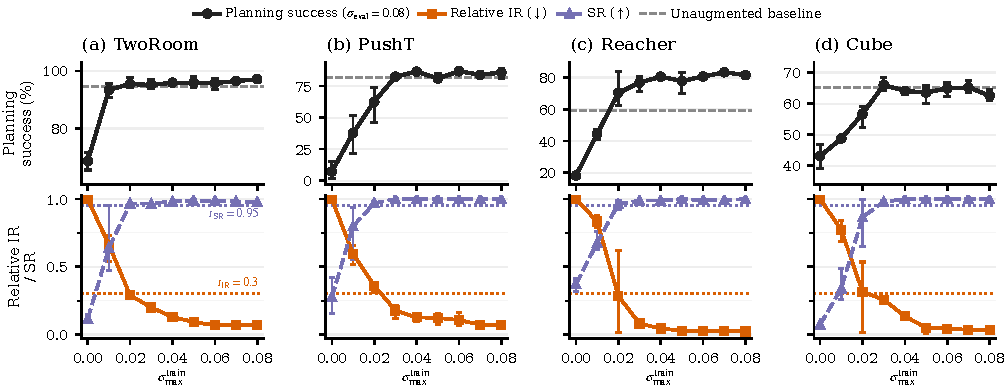
\includegraphics[width=0.94\linewidth]{fig_full_sweep_diagnostics.pdf}
\caption{Checkpoint-level planning performance and diagnostics across the
complete Gaussian-noise training sweep. Points are across-run means;
error bars span the three training runs, and success-rate axes
are scaled per task. Lower IR and higher SR are favorable.}
\label{fig:full-sweep-diagnostics}
\end{figure}

\subsection{Gaussian-Noise Performance and IR--SR Diagnostics}
\label{sec:exp-gaussian-panel}

Planning success varies with the training noise level $\sigma_{\max}$, and the
best-performing range differs across tasks
(\Cref{fig:full-sweep-diagnostics}). Reacher is a special case: augmentation
also increases clean success from $59.2\%$ to $76$--$82\%$, so its higher
success under noisy evaluation cannot be attributed to robustness alone.

Across tasks, every augmentation level that meets the success-rate criterion
has lower IR and higher SR than its matched unaugmented reference, although
neither diagnostic changes monotonically with $\sigma_{\max}$. Across the
108 LeWM checkpoint rows, 77 pass the IR threshold $\tau_{\mathrm{IR}}=0.3$.
Every checkpoint that passes the IR threshold also passes the SR threshold
$\tau_{\mathrm{SR}}=0.95$.

The evaluated PLDM sweeps show a similar qualitative pattern: better control
performance is associated with lower IR and higher SR
(Appendix~\ref{sec:appendix-A}). Both diagnostics also remain informative
under the tested blur and resize shifts
(Appendix~\ref{sec:appendix-cross-stressor}).

\subsection{IR and SR at Broader Evaluation Noise Levels}
\label{sec:exp-multiseverity-extension}

We use the broad-severity experiment to test whether checkpoints that pass the
relative-IR threshold also preserve separation between different-state
rollouts.

\begin{figure}[htbp]
\centering
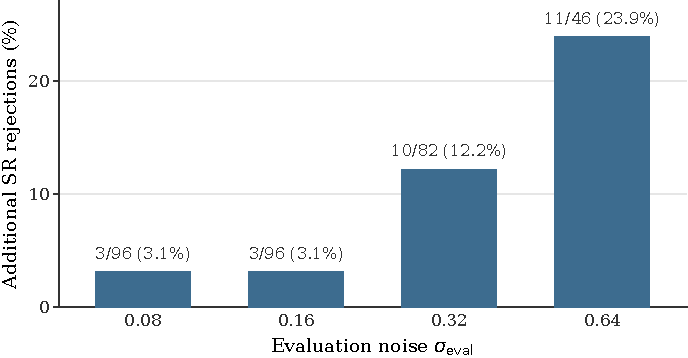
\includegraphics[width=0.46\linewidth]{fig_sr_guard_activation_by_severity.pdf}
\caption{\textbf{SR provides a distinct fixed-threshold constraint beyond
relative IR.}
Among checkpoints satisfying
$\mathrm{IR}^{\mathrm{rel}}\leq\vTwoIRThreshold$, each bar shows the
percentage rejected by $\mathrm{SR}<\vTwoSRThreshold$; annotations give the
rejection count and the number passing IR.}
\label{fig:sr-guard-activation}
\end{figure}

Among checkpoints that pass the relative-IR threshold, SR rejects
\vTwoVetoAtZeroEight{}/\vTwoIRPassAtZeroEight{} at
$\sigma_{\mathrm{eval}}=\vTwoEvalZeroEight$ and
\vTwoVetoAtZeroSixteen{}/\vTwoIRPassAtZeroSixteen{} at
$\sigma_{\mathrm{eval}}=\vTwoEvalZeroSixteen$. The rejection count increases to
\vTwoVetoAtZeroThirtyTwo{}/\vTwoIRPassAtZeroThirtyTwo{} and
\vTwoVetoAtZeroSixtyFour{}/\vTwoIRPassAtZeroSixtyFour{} at the two larger
evaluation noise levels
(\Cref{fig:sr-guard-activation}; Appendix~\ref{sec:appendix-multiseverity}).
Thus, passing IR alone does not guarantee preserved state separation,
especially as evaluation noise increases; SR provides an additional check on
this property.

\subsection{ACPC and Prediction-Error Change}\label{sec:exp-target-aligned}

We test whether eight-step ACPC under the recorded actions helps explain the
perturbation-induced prediction-error change $d=|e_{\tilde h}-e_h|$.
We use $H=8$, the longest horizon with a complete logged future for every
anchor, and analyze the unaugmented checkpoint from each task and training
run.

We estimate $d$ with ridge regression using 16-fold group cross-validation:
15 trajectory groups are used for training and the remaining group for testing,
with all samples from the same trajectory kept in one split
(Appendix~\ref{sec:appendix-p1-controls}).

The Base model uses perturbation severity, encoder distance, and one-step ACPC as the covariates for regression.
Base+Control$_8$ additionally uses the best-performing eight-step ACPC computed
with zeroed, swapped, or temporally shuffled actions. Base+ACPC$_8$ instead
uses eight-step ACPC under the recorded actions. These comparisons test whether
multi-step ACPC adds information beyond simpler diagnostics and whether that
information depends on the recorded action sequence.

\begin{figure}[H]
\centering
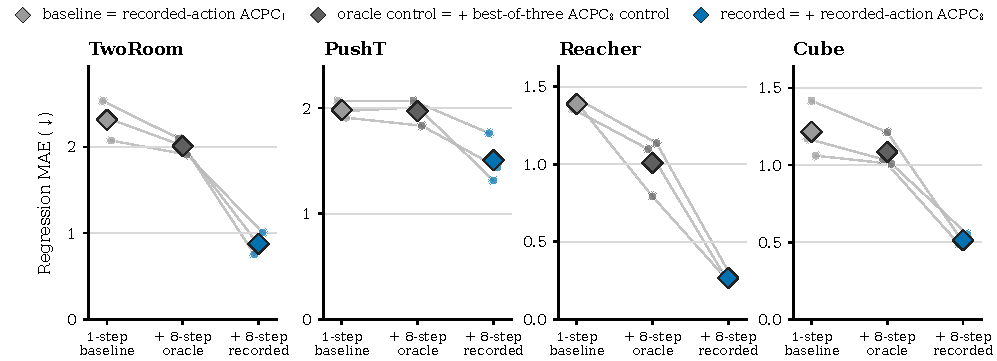
\includegraphics[width=0.90\linewidth]{fig_future_drift_three_seed_v1.pdf}
\caption{Cross-validated MAE for predicting the error drift $d$ on the
unaugmented checkpoints; lower is better.}
\label{fig:future-drift-runs}
\end{figure}

Base+ACPC$_8$ achieves the lowest cross-validated MAE in all 12 task--run
cells (\Cref{fig:future-drift-runs}). Its MAE is $55.9\pm4.7\%$ lower than
Base and $51.3\pm3.5\%$ lower than Base+Control$_8$ (mean $\pm$ sample
standard deviation across the three runs). These results show that eight-step
ACPC under the recorded actions provides information about prediction-error
change beyond both the simpler diagnostics and the tested destroyed-action
controls.

\subsection{ACPC and the Cost of CEM Plan Changes}
\label{sec:exp-planner}

A visual perturbation may cause CEM to select a different action sequence, but
a plan change alone does not indicate how consequential that change is. We
therefore test whether planner-horizon ACPC helps predict the additional
planner cost associated with selecting the perturbed-history plan.

Let $\mathbf a$ and $\tilde{\mathbf a}$ denote the final plans selected from
the clean and perturbed histories. We measure
$(C_h(\tilde{\mathbf a})-C_h(\mathbf a))_+$,
the extra cost assigned by the clean model to the perturbed-history plan, and
refer to it as \emph{CEM selection regret}, where $(x)_+=\max(x,0)$. This is a single-decision model
cost, not cumulative regret or simulator return.

We fit two ridge regression models to predict
$\log(1+\text{selection regret})$. The baseline regression uses perturbation
severity, training condition, one-step ACPC, and the clean cost gap between the best and second-best candidates. The expanded regression adds five-step ACPC,
which measures perturbation-induced divergence over the full CEM planning
horizon. For each candidate pool, ACPC is computed for every candidate action
sequence and summarized by its 90th percentile. Within each training run, both
models are trained on three tasks and tested on the held-out task, rotating
across all four tasks.
Appendix~\ref{sec:appendix-planner-protocol} gives the CEM protocol,
budget, and sample counts.

\begin{figure}[htbp]
\centering
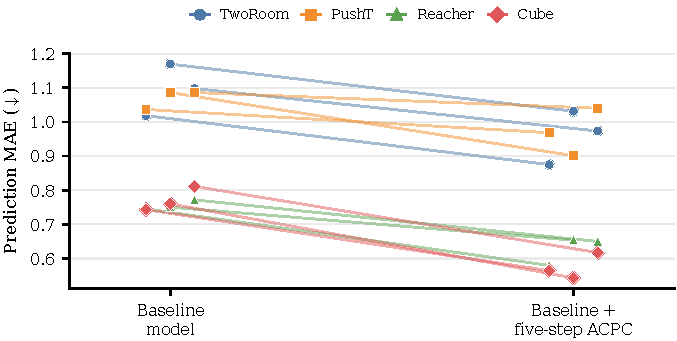
\includegraphics[width=0.64\linewidth]{fig_acpc_planner_evidence.pdf}
\caption{Adding planner-horizon ACPC improves prediction of the extra model
cost associated with changes in the plan selected by adaptive CEM.}
\label{fig:acpc-planner-evidence}
\end{figure}

Adding five-step ACPC lowers cross-task test MAE by $15.2\%$, with lower error
in all 12 task--run test cases (\Cref{fig:acpc-planner-evidence}). Thus,
planner-horizon ACPC provides information about the cost of
perturbation-induced plan changes beyond immediate perturbation sensitivity
and the clean candidate-cost gap.


\subsection{Cross-Task Checkpoint Screening}
\label{sec:exp-frozen-external}

We select the IR--SR thresholds using a subset of tasks (source tasks) and
apply them unchanged to the remaining tasks (held-out tasks). For each
held-out task, checkpoints are ordered by training noise level
$\sigma_{\max}$. We compare the lowest $\sigma_{\max}$ at which the screen
passes with the lowest $\sigma_{\max}$ at which planning performance meets the
success-rate criterion. With two or three source tasks, these two points differ
by $0.5$ grid steps on average and by at most one step, where one step
corresponds to $\Delta\sigma_{\max}=0.01$.

We also evaluate the screen as a binary classifier over the held-out
checkpoints, where passing the success-rate criterion defines the positive
class. The screen achieves balanced accuracy $0.900$, precision $0.913$, and
recall $0.953$; balanced accuracy averages the correct-classification rates
for checkpoints that do and do not meet the success-rate criterion. Full
results are reported in \Cref{tab:cross-task-all-subsets} in
Appendix~\ref{sec:appendix-cross-task}.

\section{Discussion and limitations}\label{sec:disc}

\paragraph{Scope and limitations.}

ACPC diagnoses how visual perturbations change predicted rollouts and planner
costs; it does not modify CEM. Our planner experiment therefore tests whether
ACPC reflects the extra predicted cost of a perturbation-induced plan change,
not whether ACPC-guided planning improves control.
The IR--SR screen has additional requirements: relative IR needs an unaugmented
reference, IR normalization uses observed clean transitions, and SR requires
state labels to form different-state pairs. SR is therefore limited to the
tested state distinctions, and clean performance must be checked separately.
Gaussian noise is evaluated at multiple levels, whereas blur and resize are
tested at only one level each. We also do not evaluate natural changes in
background, lighting, camera pose, or occlusion. The selected IR threshold is
at the boundary of the tested range, so larger values remain untested.

\section{Conclusion}\label{sec:conc}

ACPC measures how much a clean observation and its visually perturbed
counterpart diverge after both are rolled forward under the same action
sequence. We show that this divergence bounds changes in multi-step prediction
error and predicted planning costs. IR and SR serve complementary diagnostic
roles: IR measures clean--perturbed rollout spread, while SR checks whether
different states remain distinguishable after rollout. On LeWM, the IR--SR
checkpoint screen transfers across tasks, and both diagnostics remain
informative under blur and resize. Across the evaluated checkpoints, LeWM and
PLDM show similar trends in both IR and SR\label{sec:main-text-end}.

\clearpage
\subsection*{AI use statement}
Generative AI tools were used to assist with language editing and polishing,
information retrieval, code generation, and visualization and analysis of
experimental results. The authors reviewed all AI-assisted outputs and
checked the code and analyses for correctness. The authors take full
responsibility for the final content of the submission.

\subsection*{Reproducibility statement}
The appendix specifies tasks, perturbations, checkpoints, seeds, sampling,
normalization, thresholds, and aggregation. The anonymous supplementary
material includes the code and machine-readable results needed to reproduce
the reported figures and tables.

\acpcSaveMainCounters

\bibliographystyle{iclr2027_conference}
\bibliography{references}

%% ===========================================================================
\ifdefined\ACPCFull
  \FloatBarrier
  \appendix
  % TeX Live 2025's cleveref first aid records appendix sections as sections
% unless the section counter is explicitly aliased after \appendix.
\crefalias{section}{appendix}
\section{Proofs}\label{sec:appendix-acpc-proofs}

\paragraph{Proof of \Cref{prop:target-free-error-drift}.}
Let $u=\bar G_{\mathbf a}(E_\theta(h))$,
$v=\bar G_{\mathbf a}(E_\theta(\tilde h))$, and $y=Y_{\mathbf a}^H$. Both
errors use the same target $y$ in the weighted rollout space of
\Cref{eq:acpc-h}. The reverse triangle inequality gives
\begin{align}
|e_{\tilde h}-e_h|
&=\bigl|\,\|v-y\|_2-\|u-y\|_2\,\bigr| \\
&\le \|(v-y)-(u-y)\|_2
=\|v-u\|_2
=\mathrm{ACPC}_H(h,\tilde h,\mathbf a).
\end{align}
The one-sided error increase satisfies the same bound because
$(e_{\tilde h}-e_h)_+\le|e_{\tilde h}-e_h|$.

\paragraph{Proof of \Cref{prop:exact-cost-certificate}.}
For a single candidate, omit the index. Let $r=\|\tilde x-x\|_2$ and
$A=\mathrm{ACPC}_H(h,\tilde h,\mathbf a)$. Since $r$ is the final-step
displacement in ACPC, its definition gives
\[
\alpha_H r^2\leq A^2.
\]
Thus, $r\leq A/\sqrt{\alpha_H}$. The difference between the two squared costs
factors as
\begin{align}
|\tilde C-C|
&=\bigl|\|\tilde x-g\|_2^2-\|x-g\|_2^2\bigr| \\
&=\bigl|\langle \tilde x-x,\tilde x+x-2g\rangle\bigr| \\
&\le \|\tilde x-x\|_2\,\|\tilde x+x-2g\|_2 \\
&\le r\bigl(2\|x-g\|_2+r\bigr) \\
&\le 2\sqrt C\,\frac{A}{\sqrt{\alpha_H}}
+\frac{A^2}{\alpha_H}.
\end{align}
The first inequality follows from Cauchy--Schwarz, and the second follows from
the triangle inequality. The last inequality uses $r\leq A/\sqrt{\alpha_H}$
and $\|x-g\|_2=\sqrt C$.

\paragraph{Tightness of the prediction-error bound.}
For the prediction-error bound, let
$u$ be a unit vector, set the common target to $Y=0$, and let the two predicted
rollouts be $su$ and $tu$, where $s,t\geq0$. Then
\[
\bigl|\,\|tu\|_2-\|su\|_2\,\bigr|
=\|tu-su\|_2,
\]
so \Cref{eq:target-free-error-drift} holds with equality.

\section{Local-Geometry Case-Study Definitions}
\label{sec:appendix-local-geometry}

This supplementary case study visualizes how augmentation contracts perturbed
views relative to nearby clean histories. We use 128 logged PushT histories.
For each history, we generate one clean view and 18 perturbed views, with six
draws at each standard deviation in $\{0.01,0.04,0.08\}$. Each of the four
qualitative t-SNE panels uses a separate deterministic
projection~\citep{vandermaaten2008tsne}, so
coordinates are not compared across panels.

\begin{figure}[H]
\centering
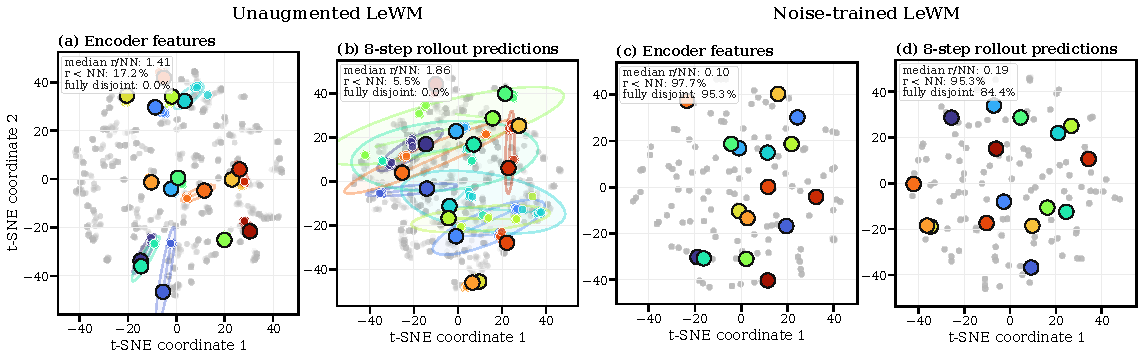
\includegraphics[width=\linewidth]{fig_local_geometry_highd_audit.pdf}
\caption{Local geometry for matched unaugmented (left) and
$\stdmax{}=0.08$ PushT checkpoints (right), at the encoder and after eight
rollout steps. Markers show clean histories and perturbed views; summaries are
computed in the original 192-dimensional space, not in t-SNE.}
\label{fig:local-geometry-highd}
\end{figure}

Without augmentation, median $r/\mathrm{NN}$ is $1.41$ at the encoder and
$1.86$ after rollout, with no fully disjoint perturbation clouds. With
augmentation, the ratios fall to $0.10$ and $0.19$, and the disjoint fractions
rise to $95.3\%$ and $84.4\%$. This is descriptive geometry, not evidence of
task-semantic separation or planning robustness.

We evaluate two representation spaces: the encoder output, denoted by
$\mathcal V=\mathrm{enc}$, and the representation after eight autoregressive
rollout steps, denoted by $\mathcal V=\mathrm{roll}$. The rollout horizon is
$H=8$ (\Cref{sec:acpc-def}). For history $i$, let
$v_{i,\mathcal V}^{(0)}$ be its clean representation and let
$v_{i,\mathcal V}^{(m)}$, $m=1,\ldots,M$ with $M=18$, be its perturbed
representations. In the rollout space, the clean and perturbed views of the
same history use the same recorded action sequence. We then define the sampled
visual radius, the distance to the nearest other clean history, and their ratio:
\begin{align}
r_{i,\mathcal V}^{\mathrm{vis}}
&=\max_{1\leq m\leq M}
\left\|v_{i,\mathcal V}^{(m)}-v_{i,\mathcal V}^{(0)}\right\|_2,
\nonumber\\
d_{i,\mathcal V}^{\mathrm{NN}}
&=\min_{j\neq i}
\left\|v_{i,\mathcal V}^{(0)}-v_{j,\mathcal V}^{(0)}\right\|_2,
\qquad
\rho_{i,\mathcal V}^{\mathrm{local}}
=\frac{r_{i,\mathcal V}^{\mathrm{vis}}}
{d_{i,\mathcal V}^{\mathrm{NN}}}.
\label{eq:local-radius-spacing}
\end{align}
The figures abbreviate $\rho_{i,\mathcal V}^{\mathrm{local}}$ as
$r/\mathrm{NN}$. A value below one means that every sampled perturbation moves
the representation by less than the distance from its clean anchor to any
other clean anchor. A value of at least one means that at least one
perturbation displacement is as large as the nearest-clean distance. This
comparison uses only distance magnitudes: it does not show that a perturbed
representation approaches or overlaps another history, and the nearest clean
history need not differ across a task-relevant state boundary.

The $r/\mathrm{NN}$ ratio considers only the perturbation radius of anchor
$i$. To account for the perturbation radii of both histories, we also compare
their enclosing balls. The ball around anchor $i$ is \emph{fully disjoint} if
it does not intersect the ball around any other anchor:
\begin{equation}
\left\|v_{i,\mathcal V}^{(0)}-v_{j,\mathcal V}^{(0)}\right\|_2
>
r_{i,\mathcal V}^{\mathrm{vis}}+r_{j,\mathcal V}^{\mathrm{vis}}
\quad\text{for every }j\neq i.
\label{eq:local-cloud-disjoint}
\end{equation}
Across the 128 anchors, we report three summaries: the median
$r/\mathrm{NN}$ ratio, the fraction with
$r_{i,\mathcal V}^{\mathrm{vis}}<d_{i,\mathcal V}^{\mathrm{NN}}$, and the
fraction satisfying the fully disjoint condition in
\Cref{eq:local-cloud-disjoint}. The second summary compares each perturbation
radius with the distance to the nearest other clean anchor. The third also
accounts for the perturbation radius around every other anchor. All three
summaries are computed in the original high-dimensional representation;
overlap between the qualitative t-SNE ellipses is not used.

These summaries are descriptive and depend on the sampled histories and
perturbation draws. They compare the encoder output and the final rollout step
but do not examine intermediate predictions. They also do not bound changes
in prediction error or planning cost; those theoretical links are provided by
pairwise ACPC in \Cref{sec:acpc-def}.

\section{Evaluation and Diagnostic Protocol}\label{sec:appendix-A}

This appendix specifies the fixed evaluation and diagnostic protocol used in
the reported results.

\paragraph{Evaluation grid.}
We evaluate LeWM on PushT, TwoRoom, Reacher, and Cube. Each checkpoint is
evaluated with seeds 42, 43, and 44, using 100 episodes per seed. The primary
evaluation adds Gaussian noise with standard deviation $0.08$ to the history
observations while keeping the goal image clean. For each task, the training
grid contains one unaugmented checkpoint and eight checkpoints trained with
full-sequence Gaussian-noise augmentation at
$\stdmax{}\in\{0.01,0.02,\ldots,0.08\}$.

\paragraph{PLDM protocol.}
PLDM is evaluated on the same four tasks and nine-checkpoint training grid as
LeWM, using the same evaluation seeds and number of logged histories. Its
diagnostics use the same clean--perturbed pairing, eight-step rollout horizon,
and SR definition. In the PLDM plots, raw IR is divided by the value of the
unaugmented PLDM checkpoint from the same task and training run.

\paragraph{PLDM results.}\label{sec:exp-pldm-diagnostics}
To test whether the diagnostics are specific to LeWM, we apply the same ACPC,
IR, and SR definitions to PLDM, which uses a different architecture and
training recipe. The evaluated PLDM sweeps show a similar qualitative pattern:
better control performance is associated with lower IR and higher SR
(\Cref{tab:pldm-all-levels}).

\begin{table}[H]
\centering
\caption{\textbf{PLDM over the complete augmented training grid.} Success and SR cells give the unaugmented three-run mean followed by the range of three-run means over all eight augmented levels $\sigma_{\max}^{\mathrm{train}}\in\{0.01,\ldots,0.08\}$; success also gives the unaugmented across-run population SD. Relative IR lists only the augmented range because its unaugmented value is one by construction. No level is selected. The grid ends at $0.08$ and therefore cannot measure an overaugmentation boundary; \Cref{fig:pldm-sweep-diagnostics} gives per-level curves and across-run ranges.}
\label{tab:pldm-all-levels}
\footnotesize
\setlength{\tabcolsep}{5.0pt}
\begin{tabular}{lccc}
\toprule
Task & \shortstack{Planning success (\%)\\unaug. $\to$ augmented range} & \shortstack{Relative IR\\augmented range} & \shortstack{SR\\unaug. $\to$ augmented range} \\
\midrule
TwoRoom & 67.1$\pm$8.0$\to$[95.7, 97.7] & [0.071, 0.440] & 0.082$\to$[0.967, 1.000] \\
PushT & 10.2$\pm$5.9$\to$[20.9, 70.3] & [0.070, 0.866] & 0.228$\to$[0.439, 1.000] \\
Reacher & 53.0$\pm$29.7$\to$[63.0, 82.2] & [0.166, 0.893] & 0.650$\to$[0.887, 1.000] \\
Cube & 45.9$\pm$1.7$\to$[50.6, 53.9] & [0.043, 0.742] & 0.170$\to$[0.637, 1.000] \\
\bottomrule
\end{tabular}
\end{table}


\begin{figure}[H]
\centering
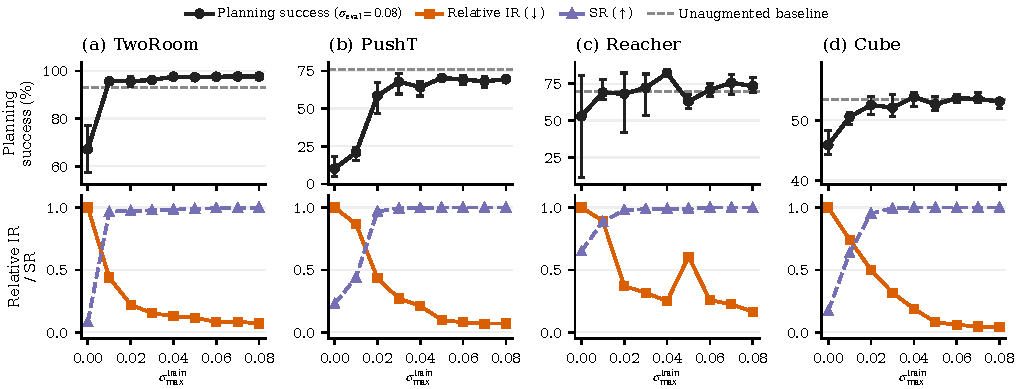
\includegraphics[width=\linewidth]{fig_pldm_sweep_diagnostics.pdf}
\caption{Complete PLDM Gaussian-noise training sweep over three runs. Curves
show three-run means and success bars span the across-run range. The summary in
\Cref{tab:pldm-all-levels} includes every augmented level rather than selecting a recovery
subset.}
\label{fig:pldm-sweep-diagnostics}
\end{figure}

\paragraph{Success-rate criterion.}
For each task and training run, let $S_0$ be the
noisy-observation success rate of the unaugmented checkpoint, and let
$S_{\max}$ be the highest noisy-observation success rate observed in
the fixed nine-checkpoint sweep. A checkpoint meets the success-rate criterion if its
noisy-observation success rate is at least
\[
S_0+0.8(S_{\max}-S_0)
\]
and its clean-observation success rate is no more than five percentage points
below that of the unaugmented checkpoint. At the task level, we call an
augmentation level recovered only when this criterion holds in at least two
of the three training runs. $S_{\max}$ is used only to scale this
recovery label; every level meeting the criterion remains part of the reported
range.

\paragraph{IR protocol.}
We compute IR separately for each task, training run, and checkpoint. To
express rollout divergence relative to the normal motion in each history, we
first compute a clean-motion scale. For anchor $i$, let
$u^{\mathrm{obs}}_{i,0}$ be the projected embedding of the final history
observation, and let $u^{\mathrm{obs}}_{i,1:H}$ be the projected embeddings of
the next $H$ observed clean frames. We define
\begin{equation}
s_i
=Q_{0.50}\!\left(
\left\{\|u^{\mathrm{obs}}_{i,k}-u^{\mathrm{obs}}_{i,k-1}\|_2
\right\}_{k=1}^{H}
\right).
\label{eq:clean-transition-scale}
\end{equation}
Thus, $s_i$ is the median displacement between consecutive clean observations,
including the transition from the final history observation to the first
future observation.

For each anchor, we generate multiple perturbation draws using the visual
shift being evaluated, with five draws for Gaussian noise. For the Gaussian-noise
experiments in \Cref{sec:exp-gaussian-panel}, we use $\sigma=0.08$; the
blur and resize experiments apply their corresponding shifts. For every draw,
we compute eight-step ACPC with uniform weights $\alpha_k=1/H$ and normalize it
by $s_i+\varepsilon_{\mathrm{norm}}$. We average the normalized values across
draws for each anchor and then take the 90th percentile (q90) across anchors.
The result is raw IR in
\Cref{eq:ir-raw}.

SR compares different-state distances with raw IR from the same checkpoint.
For the sweep plots, raw IR is divided by the value of the corresponding
unaugmented checkpoint, as defined in \Cref{eq:ir-relative}. Only the LeWM
cross-task analysis uses relative IR for threshold selection. We use
$\varepsilon_{\mathrm{norm}}=10^{-8}$ in
\Cref{eq:normalized-same-state-radius}.

Across all 108 LeWM checkpoints from the four tasks in the main Gaussian-noise
sweep, zero clean-motion scale occurred only in PushT, at one of the 100
anchors per checkpoint. For this anchor, the denominator reduces to
$\varepsilon_{\mathrm{norm}}$. Excluding it changed relative IR by at most
$0.034$, with only one checkpoint crossing each of the two fixed IR thresholds
examined ($0.1$ and $0.3$). These crossings occurred near the threshold
boundaries. The 90th-percentile aggregation prevents this single extreme value
from directly determining IR.

\Cref{tab:horizon-quantile-sensitivity} reports the results for the tested
rollout horizons and summary quantiles.

\begin{table}[H]
\centering
\caption{Horizon and quantile sensitivity of the IR reduction at fixed evaluation noise $\sigma=0.08$. Each entry is the median, over the three training runs, of the ratio between the IR of the checkpoint trained at the highest augmentation level ($\stdmax{}=0.08$) and that of the unaugmented checkpoint; lower means a larger reduction. q80, q90, and q95 denote the 80th, 90th, and 95th percentiles, respectively. These values are descriptive and do not retune any threshold.}
\label{tab:horizon-quantile-sensitivity}
\small
\setlength{\tabcolsep}{5pt}
\begin{tabular}{lccccccc}
\toprule
& \multicolumn{4}{c}{$q=0.90$ by horizon} & \multicolumn{3}{c}{$H=8$ by quantile} \\
\cmidrule(lr){2-5}\cmidrule(lr){6-8}
Task & H1 & H2 & H4 & H8 & q80 & q90 & q95 \\
\midrule
TwoRoom & 0.05 & 0.04 & 0.05 & 0.06 & 0.06 & 0.06 & 0.06 \\
PushT & 0.06 & 0.07 & 0.06 & 0.09 & 0.07 & 0.09 & 0.09 \\
Reacher & 0.02 & 0.03 & 0.03 & 0.02 & 0.02 & 0.02 & 0.02 \\
Cube & 0.04 & 0.03 & 0.04 & 0.04 & 0.03 & 0.04 & 0.04 \\
\bottomrule
\end{tabular}
\end{table}


\paragraph{SR protocol.}
SR follows \Cref{eq:sr}. We first define a local neighborhood using the
standardized logged endpoint states. Let $d_{0.35}$ be the 35th percentile of
all pairwise distances between different endpoints---that is, the q35 of all off-diagonal Euclidean distances.
This cutoff keeps the comparisons local while retaining an eligible neighbor for most anchors;
\Cref{tab:sr-labels} reports the resulting counts.

For each anchor $i$, we select the nearest history $j(i)$ that has a different
endpoint-state label and lies within distance $d_{0.35}$. If no such history
exists, the anchor is excluded from SR. We roll both histories forward under
the anchor's recorded action sequence $\mathbf a_i$. This sequence was not
generally executed by the neighboring history, but using it for both rollouts
prevents action differences from affecting the comparison. Their normalized
rollout distance is
\begin{equation}
D_i^{\mathrm{diff}}
=
\frac{
\left\|\bar G_{\mathbf a_i}(E_\theta(h_i))
-\bar G_{\mathbf a_i}(E_\theta(h_{j(i)}))\right\|_2
}{s_i+\varepsilon_{\mathrm{norm}}}.
\end{equation}
The pair counts as separated when $D_i^{\mathrm{diff}}$ is greater than raw
q90 IR plus the fixed margin $0.10$.
Prediction errors in the neighbor's rollout under the anchor's actions may
increase the measured separation.

For pairing, the endpoint state is taken after the eight observed future steps
and therefore records the state reached under that trajectory's own actions.
The dataset preprocessor standardizes each state coordinate, and neighborhood
distances use the full standardized state vector. Endpoint-state labels are
constructed by median splits of the task-specific coordinates listed in
\Cref{tab:sr-labels}, using the fixed batch of 100 endpoints generated with
anchor seed 9101. Because the logged endpoints, labels, and neighborhoods are
fixed before checkpoint evaluation, the selected pairs and eligible-anchor
counts are identical across checkpoints and training runs.

\begin{table}[H]
\centering
\caption{Endpoint-state labels used to construct SR pairs. The state is taken
at the eighth observed future step, and its coordinates are standardized using
full-dataset statistics. Counts report eligible and skipped histories among
the fixed 100 anchors. These labels define operational partitions for the
diagnostic; they are not semantic or action-relevance annotations.}
\label{tab:sr-labels}
\footnotesize
\setlength{\tabcolsep}{3pt}
\begin{tabularx}{\linewidth}{l l X r}
\toprule
Task & Logged state field (dim.) & Label construction $\ell(y)$ & Eligible / skipped \\
\midrule
TwoRoom & \code{pos\_agent} (2) & Median split of the standardized agent $x$ coordinate (\code{pos\_agent[0:1]}). & 61 / 39 \\
PushT & \code{state} (7) & Three-bit label from median splits of standardized block $x$, block $y$, and block angle (\code{state[2:5]}). & 98 / 2 \\
Reacher & \code{observation} (6) & Three-bit label from median splits of the two standardized joint velocities and their Euclidean norm (\code{observation[4:6]}). & 100 / 0 \\
Cube & \code{observation} (28) & Three-bit label from median splits of the first two standardized coordinates and $\|r\|_2$, where $r=\bar o_{0:3}-\bar o_{25:28}$. & 100 / 0 \\
\bottomrule
\end{tabularx}
\end{table}

\paragraph{Threshold grids.}
For the LeWM cross-task evaluation, we search
\[
t_{\mathrm{IR}}\in\{0.05,0.075,0.10,0.15,0.20,0.30\},
\qquad
t_{\mathrm{SR}}\in\{0.80,0.85,0.90,0.95\}.
\]
For each nonempty subset of tasks used for threshold selection, we evaluate
every threshold pair. We first minimize the mean number of augmentation-grid
steps between the first checkpoint accepted by the IR--SR screen and the
first checkpoint that meets the success-rate criterion. Remaining ties are
resolved by, in order, fewer early acceptances, fewer late acceptances, higher
balanced accuracy, a smaller $t_{\mathrm{IR}}$, and a larger
$t_{\mathrm{SR}}$.

The selected thresholds are then applied unchanged to the tasks that were not
used for their selection. Success-rate labels from those tasks and all blur
or resize results are excluded from threshold selection.

\paragraph{Reproducibility.}
The commands used to rebuild the paper figures and tables are documented in
\codebrk{paper1/scripts/README.md} and
\codebrk{tools/README\_paper1.md}. The
released machine-readable summaries are sufficient for the reader-facing
aggregation and plotting steps. Recomputing checkpoint-level diagnostics
additionally requires the released checkpoints and datasets. The summaries
record the training seeds, evaluation seeds, and protocol hashes used for each
result.

\begin{table}[H]
\centering
\caption{Recovery ranges in the original Gaussian-noise training sweep
(nine checkpoints per task: no augmentation plus eight noise levels;
\Cref{fig:full-sweep-diagnostics} shows every level). The final column lists
the contiguous training-noise ranges that meet the prespecified success-rate
criterion in \Cref{sec:bg}. It summarizes an accepted range rather than
selecting a single training strength.}
\label{tab:full-sweep-compact}
\footnotesize
\setlength{\tabcolsep}{7pt}
\begin{tabular}{lrr}
\toprule
Task & Unaugmented success (\%) & Training levels meeting criterion \\
\midrule
TwoRoom & 68.8 & 0.01--0.08 \\
PushT & 7.2 & 0.03--0.08 \\
Reacher & 18.2 & 0.03--0.08 \\
Cube & 43.1 & 0.03--0.07 \\
\bottomrule
\end{tabular}
\end{table}


\FloatBarrier
\section{Additional Multi-Severity Analysis}
\label{sec:appendix-multiseverity}

\providecommand{\vTwoNumberMacros}{tables/multiseverity_numbers}
\input{\vTwoNumberMacros}
\providecommand{\vTwoAssociationTable}{tables/table_multiseverity_associations}
\providecommand{\vTwoDecisionTable}{tables/table_multiseverity_decisions}

This section gives the aggregation and sensitivity details behind
\Cref{sec:exp-multiseverity-extension}. The broad-severity experiment is
analyzed separately from the original narrow sweep. It keeps the original
thresholds and pair construction fixed and uses continuous retention rather
than defining a new performance band.

The same \vTwoVetoAtZeroEight{} TwoRoom checkpoints account for every
additional SR rejection among IR-passing rows at
$\sigma_{\mathrm{eval}}=\vTwoEvalZeroEight$ and
$\vTwoEvalZeroSixteen$: \vTwoLowVetoAtOne{} has
$\sigma_{\max}=\vTwoTrainOne$ and \vTwoLowVetoAtOneFive{} have
$\sigma_{\max}=\vTwoTrainOneFive$. At
$\sigma_{\mathrm{eval}}=\vTwoEvalZeroThirtyTwo$, these rejections comprise
\vTwoVetoThirtyTwoTwoRoom{} TwoRoom, \vTwoVetoThirtyTwoPushT{} PushT, and
\vTwoVetoThirtyTwoReacher{} Reacher checkpoints; at
$\vTwoEvalZeroSixtyFour$, they comprise
\vTwoVetoSixtyFourTwoRoom{} TwoRoom and \vTwoVetoSixtyFourPushT{} PushT
checkpoints. No Cube checkpoint passes IR while failing SR. The conditional
rejections thus
span three tasks at $\vTwoEvalZeroThirtyTwo$ and two at
$\vTwoEvalZeroSixtyFour$, although some checkpoint rows recur across severity
slices and the conditional denominator also changes. All low-severity
rejections fall on TwoRoom, whose SR catalog uses one median split and has the
fewest eligible anchors (61 of 100; \vTwoSRLabelReference); this concentration should be
read within the scope of the tested pair catalog.

\input{\vTwoDecisionTable}
\FloatBarrier

The conditions also disagree in the other direction: at both
$\sigma_{\mathrm{eval}}=0.32$ and $0.64$,
\vTwoSROnlyPassAtZeroThirtyTwo{} and \vTwoSROnlyPassAtZeroSixtyFour{} rows,
respectively, pass SR but fail relative IR.
The reverse disagreement in
\Cref{tab:multiseverity-decision-decomposition} is expected to be possible
because the conditions use different references. Relative IR divides the raw
perturbation radius by the unaugmented checkpoint's radius at the same
severity. SR instead compares that raw radius with clean different-state
distances from the checkpoint under evaluation. The fixed-threshold results
therefore cannot be reproduced by nesting one condition inside the other.

For each task and training run, the grid contains eight training-noise maxima
and four evaluation severities. Let $x_{ij}$ denote any diagnostic or behavioral
quantity at training level $i$ and evaluation severity $j$. We remove the two
additive main effects using
\[
\widetilde{x}_{ij}
=x_{ij}-\overline{x}_{i\cdot}-\overline{x}_{\cdot j}
+\overline{x}_{\cdot\cdot}.
\]
Spearman correlations are computed over the \vTwoFactorialCellCount{} centered
cells within a single task and training run. We then average the
\vTwoRunCount{} training-run correlations within each task and weight the
\vTwoTaskCount{} tasks equally. The task ranges in
\Cref{tab:multiseverity-associations} summarize heterogeneity; they are not
confidence intervals. Double-centering leaves
$(\vTwoTrainLevelCount-1)(\vTwoEvalLevelCount-1)=\vTwoInteractionDf$
interaction degrees of freedom and imposes row- and column-sum constraints, so
the \vTwoFactorialCellCount{} cells are not treated as independent observations.

\input{\vTwoAssociationTable}
\FloatBarrier

We next relate the continuous diagnostics to same-checkpoint retention,
defined as success under noise minus clean success. After accounting for the
simple exposure ratio $-\sigma_{\mathrm{eval}}/\sigma_{\max}$, the correlations
remain positive when tasks are weighted equally: \vTwoIRAdjusted{} for IR and
\vTwoSRAdjusted{} for SR.
The adjusted IR
association is near zero on PushT (\vTwoIRAdjustedPushT{}), so the result is not
uniform across tasks. These associations do not establish
better checkpoint selection or replace evaluation of nominal model quality.

On PushT, the exposure comparator's direct task-level correlation exceeds both
diagnostics. This is why we use it as an explicit design-metadata comparator
and do not interpret the small differences among the direct aggregate values as
diagnostic superiority.

Using stress success divided by same-checkpoint clean success instead of their
percentage-point difference gives the same qualitative result. The equal-task
mean direct correlations are $\vTwoIRRatioDirect$ for lower relative IR and
$\vTwoSRRatioDirect$ for higher SR; after accounting for the exposure ratio
they are $\vTwoIRRatioAdjusted$ and $\vTwoSRRatioAdjusted$, respectively.
Every clean-success estimate is nonzero (minimum
$\vTwoMinimumCleanSuccess\%$), but ratios can still amplify changes for weak
checkpoints; we therefore keep the percentage-point difference as the primary
outcome and treat the ratio only as a sensitivity check. These are descriptive
factorial associations. The \vTwoRowCount{} rows are not independent
replicates, and the four evaluation-severity rows for a checkpoint share the
same clean-performance estimate; therefore we do not attach row-level
$p$-values or confidence intervals.


\FloatBarrier
\section{Prediction-Error Scope and Controls}\label{sec:appendix-p1-controls}

We checked \Cref{prop:target-free-error-drift} for every logged eight-step pair
and every candidate-specific five-step pair across all tasks, training runs,
and training conditions. No numerical violations occurred. This check
confirms that the implementation follows the inequality. It is not an independent statistical success count
or evidence of model quality, because the inequality holds for every correctly
computed pair.

The prediction-error and planning experiments answer different questions. The
prediction-error experiment measures how a visual perturbation changes
rollout error relative to the observed future under the recorded actions. The
planning experiment instead computes ACPC for the action candidates evaluated
by CEM and relates it to selection regret. We therefore treat the planning
analysis as separate evidence rather than infer it from the prediction-error
result (\Cref{sec:exp-planner}).

The prediction-error analysis uses only the unaugmented checkpoints.
Each history pair contributes rows at Gaussian-noise standard deviations
$\sigma\in\{0.02,0.05,0.08\}$ with two perturbation draws; zero-severity probes
serve only as identity checks.
Base+Control$_8$ reports the lowest test MAE
among the three action controls for each task and training run.
\Cref{tab:target-aligned-acpc} reports the relative reduction in
cross-validated MAE for each training run.
\Cref{tab:target-aligned-acpc-absolute} reports the corresponding MAE values
and the selected destroyed-action controls. Base+ACPC$_8$ achieves lower MAE
than both comparison models on all four tasks in every training run.

\begin{table}[!htb]
\centering
\caption{Relative reduction in out-of-group MAE from Base+ACPC$_8$ when predicting the error drift $d$ on the unaugmented checkpoints (protocol and model definitions in \Cref{sec:exp-target-aligned}). Base+Control$_8$ uses the per-cell oracle control; higher is better. The last column counts task--run cells in which Base+ACPC$_8$ is best.}
\label{tab:target-aligned-acpc}
\small
\setlength{\tabcolsep}{6pt}
\begin{tabular}{lrrc}
\toprule
Training run (seed) & vs. Base & vs. Base+Control$_8$ & Task--run cells improved \\
\midrule
3072 & 55.5\% & 51.4\% & 4/4 \\
3073 & 60.8\% & 54.8\% & 4/4 \\
3074 & 51.4\% & 47.7\% & 4/4 \\
\midrule
mean $\pm$ SD & 55.9 $\pm$ 4.7\% & 51.3 $\pm$ 3.5\% & 12/12 \\
\bottomrule
\end{tabular}
\end{table}

\begin{table}[!htb]
\centering
\caption{Out-of-group MAE (16-fold leave-one-trajectory-group-out) for predicting the error drift $d$ on the unaugmented checkpoints; lower is better, model definitions in \Cref{sec:exp-target-aligned}. ``Selected control'' is the destroyed-action control chosen by the per-cell oracle; ``paired wins'' counts the folds (of 16) in which Base+ACPC$_8$ beats Base+Control$_8$.}
\label{tab:target-aligned-acpc-absolute}
\footnotesize
\setlength{\tabcolsep}{3.2pt}
\begin{tabular}{lrrrrlc}
\toprule
Task & \shortstack{run\\(seed)} & Base & \shortstack{Base\\$+$Control$_8$} & \shortstack{Base\\$+$ACPC$_8$} & \shortstack{selected\\control} & \shortstack{paired\\wins} \\
\midrule
TwoRoom & 3072 & 2.535 & 2.099 & 0.755 & shuffled actions & 15/16 \\
TwoRoom & 3073 & 2.336 & 2.015 & 0.866 & shuffled actions & 15/16 \\
TwoRoom & 3074 & 2.075 & 1.911 & 1.006 & swapped actions & 13/16 \\
\addlinespace[1pt]
PushT & 3072 & 2.068 & 2.068 & 1.762 & shuffled actions & 11/16 \\
PushT & 3073 & 1.969 & 2.008 & 1.315 & zeroed actions & 13/16 \\
PushT & 3074 & 1.909 & 1.833 & 1.439 & zeroed actions & 13/16 \\
\addlinespace[1pt]
Reacher & 3072 & 1.358 & 1.097 & 0.288 & shuffled actions & 16/16 \\
Reacher & 3073 & 1.399 & 0.793 & 0.247 & shuffled actions & 16/16 \\
Reacher & 3074 & 1.409 & 1.136 & 0.263 & shuffled actions & 16/16 \\
\addlinespace[1pt]
Cube & 3072 & 1.171 & 1.037 & 0.489 & zeroed actions & 14/16 \\
Cube & 3073 & 1.416 & 1.212 & 0.500 & zeroed actions & 14/16 \\
Cube & 3074 & 1.061 & 1.008 & 0.552 & shuffled actions & 14/16 \\
\bottomrule
\end{tabular}
\end{table}


\FloatBarrier
\section{Cross-Task Threshold Partitions}\label{sec:appendix-cross-task}

With four tasks, there are 14 nonempty choices of tasks for threshold
selection: four single-task choices, six two-task choices, and four three-task
choices. The selected thresholds are applied to the remaining task or tasks.
Each evaluation includes all three training runs and all nine checkpoints for
every remaining task. Checkpoints are not counted as independent samples:
metrics first average the training runs within each evaluation task and then
weight the evaluation tasks equally.

When thresholds are selected using only Reacher, the procedure chooses
$(t_{\mathrm{IR}},t_{\mathrm{SR}})=(0.1,0.95)$ instead of the predominant
$(0.3,0.95)$. Both threshold pairs locate Reacher recovery within one
augmentation-grid step, but $t_{\mathrm{IR}}=0.1$ matches the Reacher onset
exactly and therefore wins the tie-break. Recovered Reacher checkpoints have
relative IR well below $0.1$, whereas the earliest recovered checkpoints on
the other tasks remain above $0.1$. The Reacher-only threshold therefore
accepts recovery on those tasks too late, by as many as five augmentation
levels.

\begin{table*}[t]
\centering
\caption{Joint IR/SR checkpoint screening with thresholds chosen on other tasks. Thresholds are selected on the threshold-selection tasks and applied unchanged to all test tasks. Metrics first average training runs within each test task and then weight tasks equally. Recovery-onset mismatch is measured in training-augmentation grid levels (one level is $0.01$ in $\stdmax{}$).}
\label{tab:cross-task-all-subsets}
\small
\setlength{\tabcolsep}{3.5pt}
\begin{tabular}{>{\raggedright\arraybackslash}p{0.17\textwidth}>{\raggedright\arraybackslash}p{0.17\textwidth}rrrrr}
\toprule
Selection tasks & Test tasks & $t_{\mathrm{IR}}$ & $t_{\mathrm{SR}}$ & BA & P / R & \shortstack{Onset mismatch\\mean / max} \\
\midrule
TwoRoom & PushT, Reacher, Cube & 0.3 & 0.95 & 0.888 & 0.884 / 0.981 & 0.3 / 1.0 \\
PushT & TwoRoom, Reacher, Cube & 0.3 & 0.95 & 0.894 & 0.902 / 0.956 & 0.6 / 1.0 \\
Reacher & TwoRoom, PushT, Cube & 0.1 & 0.95 & 0.723 & 0.906 / 0.540 & 2.9 / 5.0 \\
Cube & TwoRoom, PushT, Reacher & 0.3 & 0.95 & 0.913 & 0.950 / 0.938 & 0.6 / 1.0 \\
TwoRoom, PushT & Reacher, Cube & 0.3 & 0.95 & 0.874 & 0.853 / 1.000 & 0.3 / 1.0 \\
TwoRoom, Reacher & PushT, Cube & 0.3 & 0.95 & 0.887 & 0.873 / 0.972 & 0.3 / 1.0 \\
TwoRoom, Cube & PushT, Reacher & 0.3 & 0.95 & 0.903 & 0.925 / 0.972 & 0.3 / 1.0 \\
PushT, Reacher & TwoRoom, Cube & 0.3 & 0.95 & 0.896 & 0.901 / 0.935 & 0.7 / 1.0 \\
PushT, Cube & TwoRoom, Reacher & 0.3 & 0.95 & 0.912 & 0.952 / 0.935 & 0.7 / 1.0 \\
Reacher, Cube & TwoRoom, PushT & 0.3 & 0.95 & 0.926 & 0.972 / 0.907 & 0.7 / 1.0 \\
TwoRoom, PushT, Reacher & Cube & 0.3 & 0.95 & 0.858 & 0.802 / 1.000 & 0.3 / 1.0 \\
TwoRoom, PushT, Cube & Reacher & 0.3 & 0.95 & 0.889 & 0.905 / 1.000 & 0.3 / 1.0 \\
TwoRoom, Reacher, Cube & PushT & 0.3 & 0.95 & 0.917 & 0.944 / 0.944 & 0.3 / 1.0 \\
PushT, Reacher, Cube & TwoRoom & 0.3 & 0.95 & 0.935 & 1.000 / 0.869 & 1.0 / 1.0 \\
\bottomrule
\end{tabular}
\end{table*}


\paragraph{Sensitivity to the recovery criterion.}
CEM's random sampling introduces variation in measured success rates.
We therefore use a recovery fraction of 0.8 to allow some deviation from the
highest observed success rate. We also test fractions of 0.7 and 0.9,
reselecting thresholds on source tasks for each fraction while keeping the
clean-performance constraint unchanged. Balanced accuracy is similar at 0.7
and 0.8 and lower at 0.9 (\Cref{tab:recovery-fraction-sensitivity}).

\begin{table}[htbp]
\centering
\caption{Balanced accuracy under different recovery criteria. All test cases
are included, including one case with no accepted checkpoint at fraction 0.9
when using a single source task.}
\label{tab:recovery-fraction-sensitivity}
\small
\begin{tabular}{cccc}
\toprule
Recovery fraction & 1 source task & 2 source tasks & 3 source tasks \\
\midrule
0.7 & 0.854 & 0.895 & 0.895 \\
0.8 & 0.855 & 0.900 & 0.900 \\
0.9 & 0.779 & 0.799 & 0.813 \\
\bottomrule
\end{tabular}
\end{table}


\FloatBarrier
\section{Cross-Stressor Pairs and Boundary Cases}
\label{sec:appendix-cross-stressor}

\label{sec:exp-cross-stressor}

We test whether IR and SR remain informative under visual shifts not used for
training. For each task and training run, we compare the unaugmented checkpoint
with the checkpoint trained at $\stdmax{}=0.08$ under blur ($k=15$) and resize
(scale $0.25$), giving $4\times3\times2=24$ comparisons. IR and SR are
recomputed under each shift.

For each pair, IR improvement is
$1-\mathrm{IR}^{\mathrm{rel}}_q$, and SR improvement is the SR of the augmented
checkpoint minus that of the unaugmented checkpoint. Positive values therefore
mean lower perturbation sensitivity and better state separation, respectively.
We ask whether these diagnostic improvements agree with control performance:
a pair is considered improved if planning success under the shift increases by
at least five percentage points while clean success drops by no more than five.

IR and SR each agree with this criterion in 22 of the 24 comparisons. Their
Spearman correlations with the change in planning success are $0.854$ and
$0.913$, respectively, and remain positive when any one task is omitted
(\Cref{fig:cross-stressor-components,tab:cross-stressor-components-v1}). Thus, both diagnostics remain
informative under the tested blur and resize shifts.

Component-wise reporting avoids assigning a continuous joint score to
diagnostics with different roles.
\Cref{fig:cross-stressor-components} shows the corresponding per-task changes.

The two label disagreements are PushT run 3072 under resize and run 3074 under
blur. Each gains four success points, one below the prespecified five-point
cutoff, while both diagnostic components move in the favorable direction.

\Cref{tab:cross-stressor-diagnostic-ablation} compares recorded-action ACPC
with encoder-only, one-step rollout, and action-destroying controls.

\begin{figure}[htbp]
\centering
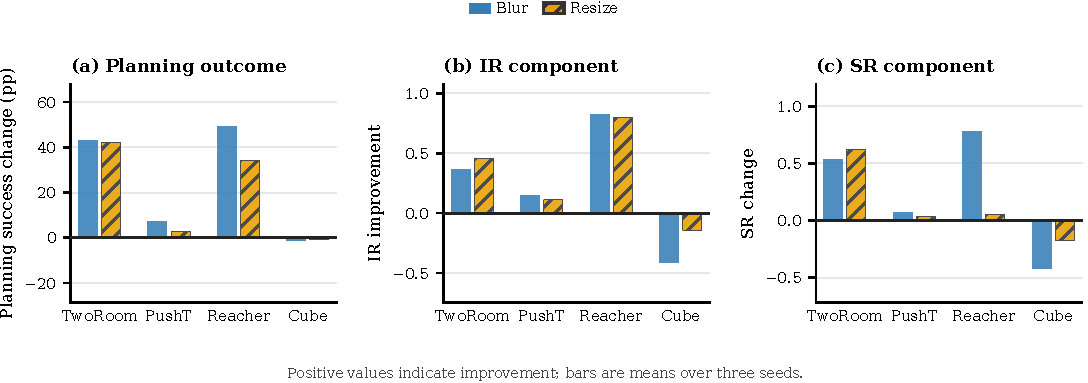
\includegraphics[width=\linewidth]{fig_cross_stressor_components_v1.pdf}
\caption{Changes from the unaugmented checkpoint to the checkpoint trained at $\stdmax{}=0.08$ under
blur and resize. Panels show (a) planning-success change in percentage points,
(b) IR improvement $1-\mathrm{IR}^{\mathrm{rel}}_q$, and (c) SR change. Bars
are means across three training runs, and positive
values indicate improvement.}
\label{fig:cross-stressor-components}
\end{figure}

\begin{table}[H]
\centering
\caption{Descriptive cross-stressor component summary. IR improvement is $1-\mathrm{IR}_{\rm rel}$ because the base value is 1; SR change is endpoint SR minus base SR. Spearman values correlate each component change with planning-success change. The leave-one-task-out (LOTO) range is obtained by omitting each task in turn and recomputing the pooled Spearman correlation. Binary agreement compares a positive component change with the prespecified positive behavior label. The final cell gives the 2.5th--97.5th percentiles from exact enumeration of all $4^4=256$ ordered task-cluster resamples, using linear interpolation. This is a sensitivity distribution, not a new-task population CI; the 24 paired rows are not IID.}
\label{tab:cross-stressor-components-v1}
\scriptsize
\setlength{\tabcolsep}{4pt}
\begin{tabular}{lrrrrl}
\toprule
Scope & $n$ & $\rho_{\rm IR}$ & $\rho_{\rm SR}$ & \shortstack{binary agreement\\IR / SR} & \shortstack{cluster-resampling\\sensitivity} \\
\midrule
Pooled & 24 & 0.854 & 0.913 & 0.917 / 0.917 & \shortstack{IR: [0.263, 0.950]\\SR: [0.352, 0.929]} \\
Blur & 12 & 0.874 & 0.953 & 0.917 / 0.917 & -- \\
Resize & 12 & 0.748 & 0.846 & 0.917 / 0.917 & -- \\
\midrule
TwoRoom & 6 & 0.543 & 0.543 & 1.000 / 1.000 & -- \\
PushT & 6 & 0.464 & 0.603 & 0.667 / 0.667 & -- \\
Reacher & 6 & 0.886 & 0.886 & 1.000 / 1.000 & -- \\
Cube & 6 & -0.086 & -0.543 & 1.000 / 1.000 & -- \\
\midrule
LOTO range & 18 & [0.720, 0.911] & [0.846, 0.901] & -- & -- \\
\bottomrule
\end{tabular}
\end{table}


\begin{table}[H]
\centering
\caption{Diagnostic ablation on 24 paired blur/resize endpoints. Each metric predicts improvement when its endpoint-to-reference ratio is below one; no threshold is fitted or transferred. Spearman correlation relates diagnostic improvement, defined as one minus this ratio, to planning-success change. Correct/24 and BA compare the predicted sign with the prespecified behavioral label. The LOTO range recomputes pooled Spearman after omitting each task; the 24 pairs are clustered within four tasks.}
\label{tab:cross-stressor-diagnostic-ablation}
\small
\setlength{\tabcolsep}{4pt}
\begin{tabular}{lcccc}
\toprule
Diagnostic & Spearman & Correct / 24 & BA & LOTO Spearman range \\
\midrule
Encoder only & 0.859 & 20 & 0.778 & [0.725, 0.901] \\
One-step rollout & 0.738 & 20 & 0.778 & [0.454, 0.877] \\
Zero actions & 0.805 & 21 & 0.833 & [0.626, 0.877] \\
Cross-anchor action shuffle & 0.780 & 21 & 0.833 & [0.586, 0.869] \\
Temporal action shuffle & 0.844 & 22 & 0.889 & [0.678, 0.923] \\
Recorded-action ACPC & 0.854 & 22 & 0.889 & [0.720, 0.911] \\
\bottomrule
\end{tabular}
\end{table}


\FloatBarrier
\section{Local Sensitivity under Gaussian Noise}
\label{sec:appendix-local-sensitivity}

To relate ACPC under Gaussian noise to local model sensitivity, consider a
small isotropic perturbation $\delta x\sim\mathcal N(0,\sigma^2 I)$. Let $J_E$
and $J_G$ be the Jacobians of the encoder and rollout map, evaluated along the
clean input. A first-order expansion gives
\[
\Delta G=J_GJ_E\,\delta x+o(\|\delta x\|_2).
\]
Writing $A=J_GJ_E$ and using
$\mathbb E[\delta x\delta x^\top]=\sigma^2I$, we obtain
\begin{equation}
\mathbb E\!\left[\|A\delta x\|_2^2\right]
=\operatorname{tr}\!\left(
A\,\mathbb E[\delta x\delta x^\top]A^\top
\right)
=\sigma^2\operatorname{tr}(AA^\top)
=\sigma^2\|A\|_F^2,
\label{eq:local-gaussian-sensitivity}
\end{equation}
Therefore, for small $\sigma$,
\[
\mathbb E[\|\Delta G\|_2^2]
\approx \sigma^2\|J_GJ_E\|_F^2.
\]
The squared Frobenius norm of the composed Jacobian thus measures how strongly
the encoder--rollout path locally amplifies Gaussian observation noise.
Jacobian Frobenius norms have previously been used to measure and regularize
local representation sensitivity~\citep{rifai2011contractive}. We estimate
\[
\|J_GJ_E\|_F^2
=\operatorname{tr}\!\left[(J_GJ_E)^\top(J_GJ_E)\right]
\]
with Rademacher probes and the Hutchinson
estimator~\citep{hutchinson1989stochastic}. Jacobian--vector products compute
these estimates without constructing the full Jacobian. In every task, both
the finite-difference and Jacobian-based estimates are lower for the
noise-augmented checkpoint (\Cref{fig:local-gaussian-sensitivity}). This result
is consistent with Gaussian-noise augmentation reducing ACPC by lowering the
local sensitivity of the encoder--rollout path. The analysis applies only near
the evaluated inputs and does not provide a global robustness guarantee.

\begin{figure}[t]
\centering
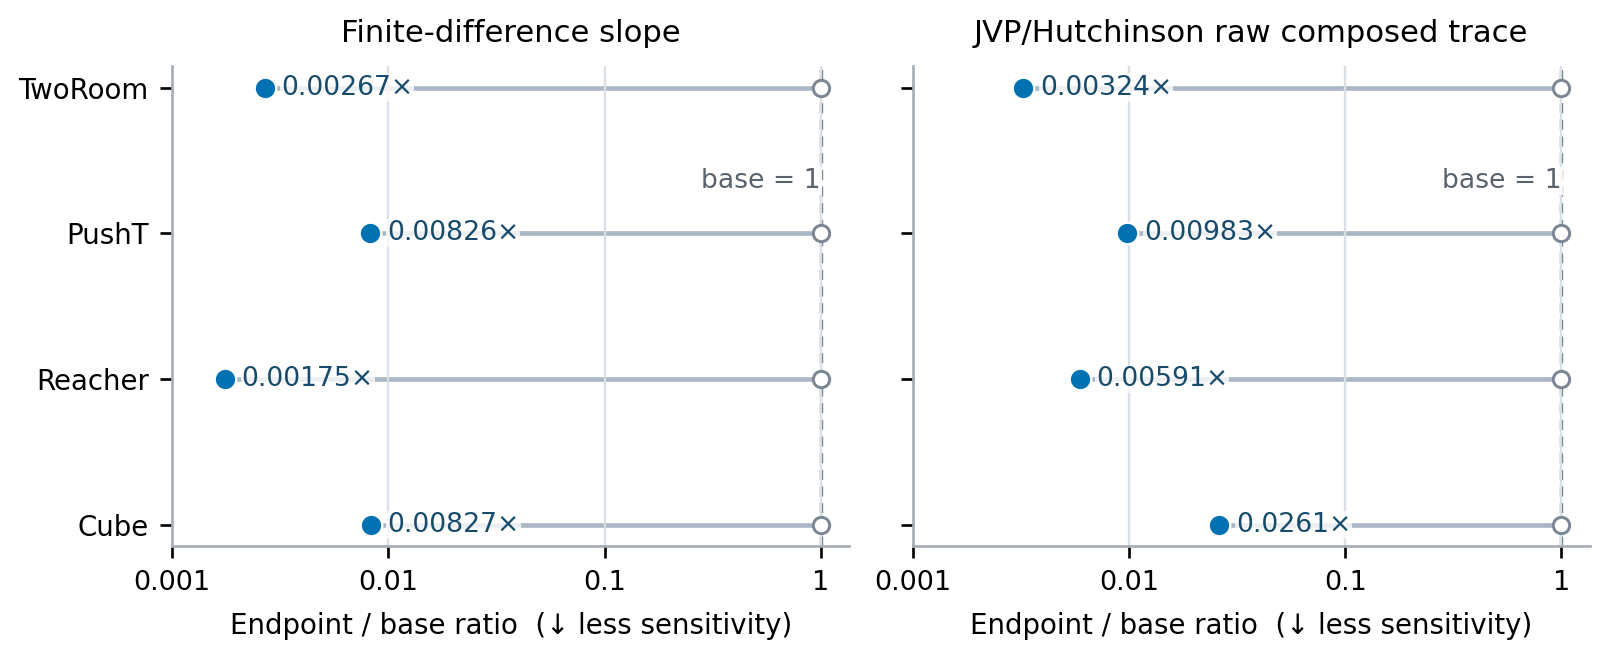
\includegraphics[width=0.88\linewidth]{fig_gaussian_sensitivity_main.png}
\caption{Ratio of local sensitivity for the Gaussian-noise-augmented
checkpoint to that of the unaugmented checkpoint. We report a
finite-difference estimate and a JVP-based Hutchinson estimate of the composed
Jacobian's squared Frobenius norm. Both estimates are below one for every task,
indicating lower local sensitivity after augmentation. These local
measurements do not establish task performance or global robustness.}
\label{fig:local-gaussian-sensitivity}
\end{figure}

\FloatBarrier
\section{Adaptive-CEM Selection Regret}
\label{sec:appendix-planner-protocol}

The selection-regret analysis does not use task-success labels. We evaluate
the unaugmented and $\stdmax{}=0.08$ checkpoints from every task and training
run. For each checkpoint, we use 100 histories and apply perturbations at
severities $0.02$, $0.05$, and $0.08$. Each clean or perturbed CEM run uses 64
candidate action sequences, eight elite candidates, eight iterations, and a
five-step prediction horizon. The paired runs start from the same proposal and
use the same random samples, but each run updates its proposal using its own
elite candidates.

The planner uses the squared distance between the predicted endpoint and the
goal embedding:
\[
C_j=\|x_j-g\|_2^2.
\]

For each CEM run, we compute ACPC for every candidate under that candidate's
action sequence. We summarize the candidate pool by the q90 ACPC at horizons
one and five. Let $\mathbf a$ be the plan selected from the clean history and
$\tilde{\mathbf a}$ the plan selected from its perturbed counterpart. The
regression target is the extra predicted cost of the perturbed-history plan
when both plans are evaluated from the clean history:
\[
\bigl[C_h(\tilde{\mathbf a})-C_h(\mathbf a)\bigr]_+.
\]

Within each training run, we fit ridge regressions on three tasks and evaluate
them on the remaining task, rotating through all four choices.
Each regression feature is standardized using the mean and standard deviation
computed from the three training tasks. The same values are used to standardize
features from the remaining test task. The target is
$\log(1+\text{selection regret})$, without further standardization. MAE is
computed on this scale and averaged equally across the four test tasks.
The relative MAE reduction is computed separately for each
training run before reporting the mean and sample standard deviation across
the three runs. This experiment evaluates whether ACPC reflects the model-cost
effect of a CEM selection change; it does not evaluate simulator return.

\Cref{tab:regression-target-scales} summarizes the target values predicted in
\Cref{sec:exp-target-aligned,sec:exp-planner}.
\begin{table}[H]
\centering
\caption{Summary statistics of the regression targets. The targets are
prediction-error change $d$ in \Cref{sec:exp-target-aligned} and
$\log(1+\text{selection regret})$ in \Cref{sec:exp-planner}.
Each task includes 288 and 1,800 samples, respectively, pooled across the
three training runs. SD denotes the standard deviation of target values,
not uncertainty in the mean.}
\label{tab:regression-target-scales}
\small
\begin{tabular}{lrrrr}
\toprule
& \multicolumn{2}{c}{Prediction-error change $d$}
& \multicolumn{2}{c}{$\log(1+\text{selection regret})$} \\
\cmidrule(lr){2-3}\cmidrule(lr){4-5}
Task & Mean & SD & Mean & SD \\
\midrule
TwoRoom & 8.756 & 6.518 & 2.123 & 2.188 \\
PushT & 6.725 & 5.653 & 2.170 & 2.077 \\
Reacher & 8.335 & 5.666 & 2.080 & 2.312 \\
Cube & 9.772 & 6.900 & 2.189 & 2.243 \\
\bottomrule
\end{tabular}
\end{table}


\fi
\end{document}
